\documentclass[a4paper,12pt]{article}

\documentclass[a4paper,12pt]{article}

%%% Работа с русским языком
\usepackage{cmap}					% поиск в PDF
\usepackage{mathtext} 				% русские буквы в формулах
\usepackage[T2A]{fontenc}			% кодировка
\usepackage[utf8]{inputenc}			% кодировка исходного текста
\usepackage[russian,english]{babel}	% локализация и переносы
\usepackage{indentfirst}            % красная строка в первом абзаце
\frenchspacing                      % равные пробелы между словами и предложениями

%%% Дополнительная работа с математикой
\usepackage{amsmath,amsfonts,amssymb,amsthm,mathtools} % пакеты AMS
\usepackage{icomma}                                    % "Умная" запятая

%%% Свои символы и команды
\usepackage{centernot} % центрированное зачеркивание символа
\usepackage{stmaryrd}  % некоторые спецсимволы

\usepackage{ifthen}

\renewcommand{\epsilon}{\ensuremath{\varepsilon}}
\renewcommand{\phi}{\ensuremath{\varphi}}
\renewcommand{\kappa}{\ensuremath{\varkappa}}
\renewcommand{\le}{\ensuremath{\leqslant}}
\renewcommand{\leq}{\ensuremath{\leqslant}}
\renewcommand{\ge}{\ensuremath{\geqslant}}
\renewcommand{\geq}{\ensuremath{\geqslant}}
\renewcommand{\emptyset}{\ensuremath{\varnothing}}

\DeclareMathOperator{\sgn}{sgn}
\DeclareMathOperator{\ke}{Ker}
\DeclareMathOperator{\im}{Im}
\DeclareMathOperator{\re}{Re}

\newcommand{\N}{\mathbb{N}}
\newcommand{\Z}{\mathbb{Z}}
\newcommand{\Q}{\mathbb{Q}}
\newcommand{\R}{\mathbb{R}}
\newcommand{\Cm}{\mathbb{C}}
\newcommand{\F}{\mathbb{F}}
\newcommand{\id}{\mathrm{id}}

\newcommand{\imp}[2]{
	(#1\,\,$\ra$\,\,#2)\,\,
}
\newcommand{\System}[1]{
	\left\{\begin{aligned}#1\end{aligned}\right.
}
\newcommand{\Root}[2]{
	\left\{\!\sqrt[#1]{#2}\right\}
}

\renewcommand\labelitemi{$\triangleright$}

\let\bs\backslash
\let\Lra\Leftrightarrow
\let\lra\leftrightarrow
\let\Ra\Rightarrow
\let\ra\rightarrow
\let\La\Leftarrow
\let\la\leftarrow
\let\emb\hookrightarrow

%%% Перенос знаков в формулах (по Львовскому)
\newcommand{\hm}[1]{#1\nobreak\discretionary{}{\hbox{$\mathsurround=0pt #1$}}{}}

%%% Работа с картинками
\usepackage{graphicx}    % Для вставки рисунков
\setlength\fboxsep{3pt}  % Отступ рамки \fbox{} от рисунка
\setlength\fboxrule{1pt} % Толщина линий рамки \fbox{}
\usepackage{wrapfig}     % Обтекание рисунков текстом

%%% Работа с таблицами
\usepackage{array,tabularx,tabulary,booktabs} % Дополнительная работа с таблицами
\usepackage{longtable}                        % Длинные таблицы
\usepackage{multirow}                         % Слияние строк в таблице

%%% Теоремы
\theoremstyle{plain}
\newtheorem{theorem}[equation]{Theorem}
\newtheorem{lemma}[equation]{Lemma}
\newtheorem{proposition}[equation]{Proposition}
\newtheorem*{exercise}{Exercise}
\newtheorem*{problem}{Problem}

\theoremstyle{definition}
\newtheorem{definition}[equation]{Definition}
\newtheorem*{corollary}{Corollary}
\newtheorem*{note}{Note}
\newtheorem*{reminder}{Reminder}
\newtheorem*{example}{Example}

\theoremstyle{remark}
\newtheorem*{solution}{Solution}

%%% Оформление страницы
\usepackage{extsizes}     % Возможность сделать 14-й шрифт
\usepackage{geometry}     % Простой способ задавать поля
\usepackage{setspace}     % Интерлиньяж
\usepackage{enumitem}     % Настройка окружений itemize и enumerate
\setlist{leftmargin=25pt} % Отступы в itemize и enumerate

\geometry{top=25mm}    % Поля сверху страницы
\geometry{bottom=30mm} % Поля снизу страницы
\geometry{left=20mm}   % Поля слева страницы
\geometry{right=20mm}  % Поля справа страницы

\setlength\parindent{0pt}         % Устанавливает длину красной строки 0pt
\linespread{1.3}                  % Коэффициент межстрочного интервала
%\setlength{\parskip}{0.5em}      % Вертикальный интервал между абзацами
%\setcounter{secnumdepth}{0}      % Отключение нумерации разделов
%\setcounter{section}{-1}         % Нумерация секций с нуля
\usepackage{multicol}			  % Для текста в нескольких колонках
\usepackage{soulutf8}             % Модификаторы начертания

%%% Содержаниие
\usepackage{tocloft}
\tocloftpagestyle{main}
%\setlength{\cftsecnumwidth}{2.3em}
%\renewcommand{\cftsecdotsep}{1}
%\renewcommand{\cftsecpresnum}{\hfill}
%\renewcommand{\cftsecaftersnum}{\quad}

%%% Шаблонная информация для титульного листа
\newcommand{\CourseName}{Introduction to Calculus}
\newcommand{\FullCourseNameFirstPart}{\so{INTRODUCTION TO CALCULUS}}
\newcommand{\SemesterNumber}{I}
\newcommand{\LecturerInitials}{Nikolay Gusev}
\newcommand{\CourseDate}{fall 2022}
\newcommand{\AuthorInitials}{Danil Klishch}
\newcommand{\VKLink}{https://vk.com/dan.klishch}
\newcommand{\GithubLink}{https://github.com/daniild71r/lectures_tex_club}

%%% Колонтитулы
\usepackage{titleps}
\newpagestyle{main}{
	\setheadrule{0.4pt}
	\sethead{\CourseName}{}{\hyperlink{intro}{\;Back to table of contents}}
	\setfootrule{0.4pt}                       
	\setfoot{MIPT, \CourseDate}{}{\thepage} 
}
\pagestyle{main}

%%% Нумерация уравнений
\makeatletter
\def\eqref{\@ifstar\@eqref\@@eqref}
\def\@eqref#1{\textup{\tagform@{\ref*{#1}}}}
\def\@@eqref#1{\textup{\tagform@{\ref{#1}}}}
\makeatother                      % \eqref* без гиперссылки
\numberwithin{equation}{subsection}  % Нумерация вида (номер_секции).(номер_уравнения)
\mathtoolsset{showonlyrefs=false} % Номера только у формул с \eqref{} в тексте.

%%% Гиперссылки
\usepackage{hyperref}
\usepackage[usenames,dvipsnames,svgnames,table,rgb]{xcolor}
\hypersetup{
	unicode=true,            % русские буквы в раздела PDF
	colorlinks=true,       	 % Цветные ссылки вместо ссылок в рамках
	linkcolor=black!15!blue, % Внутренние ссылки
	citecolor=green,         % Ссылки на библиографию
	filecolor=magenta,       % Ссылки на файлы
	urlcolor=NavyBlue,       % Ссылки на URL
}

%%% Графика
\usepackage{tikz}        % Графический пакет tikz
\usepackage{tikz-cd}     % Коммутативные диаграммы
\usepackage{tkz-euclide} % Геометрия
\usepackage{stackengine} % Многострочные тексты в картинках
\usetikzlibrary{angles, babel, quotes}

%%% Мои кастомные команды
\newcommand{\df}[2]{\begin{definition}\textit{#1} -- #2\end{definition}}

\newcommand{\abs}[1]{\left\lvert #1 \right\rvert}
\newcommand{\grad}{\mathrm{grad}\:}
\newcommand{\dlta}{\text{d}}
\newcommand{\thus}{\;\Rightarrow\;}
\newcommand{\isconst}{=\text{const}}

\newcommand{\defeq}{\vcentcolon=}
\newcommand{\defev}{\stackrel{\Delta}{\Longleftrightarrow}}
\newcommand{\deriv}[3][1]{%
	\ifthenelse{#1>1}{%
		\frac{\dlta^{#1} {#2}}{\dlta {#3}^{#1}}
	}{%
		\frac{\dlta {#2}}{\dlta {#3}}
	}%
}
\newcommand{\vc}[3]{
	\ensuremath{\begin{pmatrix} #1 \\ #2 \\ #3 \end{pmatrix}}
}
\newcommand{\vb}[2]{
	\ensuremath{\begin{pmatrix} #1 \\ #2 \end{pmatrix}}
}
\newcommand{\fnis}[1]{#1{:}\;}
\newcommand{\RR}{\mathbb{R}}
\newcommand{\NN}{\mathbb{N}}
\newcommand{\sconstr}{\;\vert\;}
\newcommand{\diag}{{\rm diag}}

\newcommand{\floor}[1]{\left\lfloor#1\right\rfloor}
\newcommand{\ceil}[1]{\left\lceil#1\right\rceil}


%%% Всю шаблонную информацию можно менять тут
\newcommand{\FullCourseNameFirstPart}{\so{КРАТНЫЕ ИНТЕГРАЛЫ И}}
\newcommand{\FullCourseNameSecondPart}{\so{ТЕОРИЯ ПОЛЯ}}
\newcommand{\SchoolName}{ФПМИ}
\newcommand{\TrackName}{ПМИ, ИВТ, КТ, РАНХиГС}
\newcommand{\SemesterNumber}{III}
\newcommand{\LecturerInitials}{Лукашов Алексей Леонидович}
\newcommand{\AutherInitialsFirst}{Климов Ярослав}
\newcommand{\AutherInitialsSecond}{Ильдаров Адам}
\newcommand{\AutherInitialsThird}{Евдокимов Егор}
\newcommand{\VKLinkFirst}{https://vk.com/klimov_yaroslav}
\newcommand{\VKLinkSecond}{https://vk.com/adamildarov}
\newcommand{\VKLinkThird}{https://vk.com/ea_evdokimov}
\newcommand{\OverleafLink}{https://www.overleaf.com/read/thzfwhhyghfn}
\newcommand{\GithubLink}{https://github.com/MIPT-Group/Lectures_Tex_Club}

\newcommand{\CourseName}{Кратные интегралы и теория поля} %  Используется в преамбуле для создания названия предмета в верхнем контитуле   
\newcommand{\CourseDate}{2020}           %  Используется в преамбуле для создания даты в нижнем контитуле и в title_page

%\includeonly{lectures/lect05,lectures/lect06}  % Чтобы скомпилировать только часть лекций

\begin{document}
    \begin{titlepage}
	\clearpage\thispagestyle{empty}
	\centering
	
	\textit{Федеральное государственное автономное учреждение \\
		высшего образования}
	\vspace{0.5ex}
	
	\textbf{Московский физико-технический институт
    \\
    (национальный исследовательский университет)
    \\
     КЛУБ ТЕХА ЛЕКЦИЙ}
	\vspace{20ex}
	
	\rule{\linewidth}{0.5mm}
	{\textbf{\FullCourseNameFirstPart}}
	\\
	{\textbf{\FullCourseNameSecondPart}}
	\rule{\linewidth}{0.5mm}
	
	\SemesterNumber\ СЕМЕСТР
	\\
	Физтех-школа: \textit{\SchoolName}
	\\
	Направление: \textit{\TrackName}
	\\
	Лектор: \textit{\LecturerInitials}
	\vspace{1ex}
	
	\begin{figure}[!ht]
		\centering
		\includegraphics[width=0.6\textwidth]{logo_LTC}
	\end{figure}
\begin{flushright}
	\noindent
	Автор(ы): \href{\VKLink}{\textit{\AutherInitials}}
	\\
	\href{\OverleafLink}{\textit{Проект на overleaf}}
	\\
	\href{\GithubLink}{\textit{Проект на github}} 
\end{flushright}
	
	\vfill
	Долгопрудный, \CourseDate\ год.
	\pagebreak
	
\end{titlepage}
    \newpage
    \hypertarget{intro}{}
    \tableofcontents
    \newpage
    \begin{flushright}
    \textit{Лекция 1 (от 07.09)}
\end{flushright}
\section{$\S 1.$ Комплексные числа}
\Def
Пусть $z = \left( x;y \right) \in \RR^2$. Пусть определены операции:
\begin{enumerate}
    \item \textbf{Сложение:} $z_1 + z_2 = \left( x_1+x_2; y_1+y_2 \right)$
    \item \textbf{Умножение на действительное число:} $\lambda z = \left(\lambda
        x, \lambda y \right)$
    \item \textbf{Расстояние:} $\rho(z_1, z_2) = \left| \left| z_1 - z_2 \right|
    \right| = \sqrt{\left( x_1 - x_2 \right)^2 + (y_1 - y_2)^2}$
\end{enumerate}
Добавим операцию
умножения друг на друга:
\begin{align*}
  & z_1 \cdot z_2 = \left( x_1 \cdot x_2 - y_1 \cdot y_2; x_1 \cdot y_2 + x_2 \cdot y_1 \right)
\end{align*}
Будем называть это \textbf{комплексными числами} $\CC$.
\\
Пусть $1 \sim (1; 0)$~--- \textbf{единица}, $i \sim (0;1)$~--- \textbf{мнимая
  единица}.
\\
Тогда $z = 1 \cdot x + i \cdot y \Leftrightarrow z = x + iy$~---
\textbf{алгебраическая запись}.
\\
Назовем $x = \Real z$ \textbf{действительной частью}, $y =
\Img z$~--- \textbf{мнимой}.
\\
\textbf{Сопряженным} к $z = x+iy$ называем $\bar{z} = x-iy$,
\textbf{модулем}~--- выражение $\left| z \right| = \sqrt{x^2+y^2}$. Легко
видеть, что $z\bar{z} = \left| z \right|^2$, полагая $i^2 = -1$.
\\
Можно представлять комплексные числа в виде $x = r \cos \varphi$, $y = r \sin
\varphi$, называя $r$ \textbf{модулем}, $\varphi$ \textbf{аргументом}, а $\arg z
\in (-\pi; \pi]$~--- одно из таких $\varphi$~--- \textbf{главным аргументом}.
Также \textbf{аргументом} называется множество $\Arg z = \left\{ \arg z + 2\pi k
    \mid k \in \ZZ \right\}$.
\\
Видим, что
\begin{align*}
  & z = \left| z \right|\cos \varphi + i \left| z \right|\sin \varphi = \left| z \right|\left( \cos \varphi + i \sin \varphi \right)
\end{align*}
Введем \textbf{комплексную экспоненту}~--- $e^{i\varphi} = \cos \varphi + i \sin
\varphi$, тогда $z = \left| z \right|e^{i\varphi}$.
\\
Для произведения тогда выполняется
\begin{align*}
  & z_1z_2 = \left| z_1 \right|\left( \cos \varphi_1 + i \sin \varphi_2 \right)\left| z_2 \right|\left( \cos \varphi_2 + i \sin \varphi_2 \right) = \left| z_1 \right|\cdot \left| z_2 \right| \left( \cos \left( \varphi_1+\varphi_2 \right) + i \sin \left( \varphi_1+\varphi_2 \right)\right)
\end{align*}
\begin{align*}
  & \left|z_1z_2\right| = \left| z_1 \right|\cdot \left| z_2 \right|
\end{align*}
\begin{align*}
  & \Arg(z_1z_2) = \Arg z_1 + \Arg z_2
\end{align*}
\textbf{Суммой Минковского} называется множество $A+B = \sets{a+b \mid a\in A, \
  b \in B}$.
\\
На комплексных числах определено \textbf{деление} на $z\neq 0$: $z_1z = z_2
\Rightarrow z = \dst \frac{z_2}{z_1}$; если $z_2=1$, то $z = \dst \frac{1}{z_1}
= z_1^{-1}$.
\\
Нахождение частного эквивалентно решению системы
\begin{align*}
  & \left\{ \begin{matrix}
          x_1x-y_1y=x_2 \\
          y_1x+x_1y = y_2
      \end{matrix} \right.
\end{align*}
Это можно выразить как
\begin{align*}
  & z = \frac{\bar{z_1}z_2}{\left| z_1 \right|^2} = \frac{\left| z_2 \right|e^{i \varphi_2}}{\left| z_1 \right| e^{i \varphi_1}} = \frac{\left| z_2 \right|}{\left| z_1 \right|}e^{i\left( \varphi_2-\varphi_1 \right)}
\end{align*}
Зная, что $e^{i \varphi_1}e^{i \varphi_2} = e^{i\left( \varphi_1+\varphi_2
  \right)}$, можем записать \textbf{формулу Муавра}:
\begin{align*}
  & \forall n \in \NN \ z^n = \left| z \right|^ne^{i n \varphi} 
\end{align*}
Также определена операция \textbf{извлечения корня} из $z^n = a \neq 0$.
Полагаем $z=re^{i\varphi}$, $a = \left| a \right|e^{i\alpha}$. Тогда $r^n =
\left| \alpha \right|$, а $n \varphi = \alpha + 2 \pi k, \ k \in \ZZ$. Отсюда $r
= \sqrt[n]{\left| a \right|}$, $\varphi_k = \dst \frac{\alpha+2\pi k}{n}$. тогда
определим корень как
\begin{align*}
  & \sets{\sqrt[n]{a}} = \sets{\sqrt[n]{\left| a \right|}\left( \cos \frac{\alpha + 2 \pi k}{n} + i \sin \frac{\alpha + 2 \pi k}{n} \right)\mid k \in \{0, \dots, n-1\}}
\end{align*}
\Example
\begin{align*}
  & \sets{\sqrt[4]{i}} = \sets{\exp\left( i \frac{\dst \frac{\pi}{2} + 2 \pi k}{4} \right)\mid k \in \{0, \dots, 3\}}
\end{align*}
\section{$\S 2.$ Последовательность. Предел. Ряды. Функции. Расширенная
  комплексная плоскость}
\Def
\textbf{Окрестностью} назовем $B_r(z_0) = \left\{ z \in \CC: \left| z-z_0
    \right| < r \right\}$. \textbf{Проколотой окрестностью} назовем
$\os{\circ}{B}_r(z_0) = \left\{ z \in \CC: 0 < \left| z-z_0 \right| < r
\right\}$. \textbf{Замкнутой окрестностью} назовем $\bar{B}_r(z_0) = \left\{ z
    \in \CC: \left| z-z_0\right| \leq r \right\}$.
\Def
Множество $\left\{ z_n \right\}_{n=1}^\infty$, $z_n  = x_n + iy_n$ называется
\textbf{последовательностью}.
\Def
Число $A \in \CC$ называется \textbf{пределом последовательности $z_n$} (пишем
$\dst \lim_{n \to \infty}z_n = A$) тогда и только тогда, когда выполняется
\begin{equation}\label{(2.1)}
    \forall \varepsilon > 0 \ \exists N(\varepsilon):\ \forall n \geq N(\varepsilon)\in \NN \hookrightarrow z_n \in B_{\varepsilon}(A)
\end{equation}
\asm
\begin{align*}
  & \exists \lim_{n \to \infty}z_n = A = a+ib \Leftrightarrow \left\{ \begin{matrix}
          \dst \lim_{n \to \infty}x_n = a \\
          \dst \lim_{n \to \infty}y_n = b
      \end{matrix} \right.
\end{align*}
\pr Докажем в обе стороны.
\begin{itemize}
    \item $\Rightarrow$:
    \begin{align*}
      & \left| x_n - a \right| \leq \left| z_n - A \right| < \varepsilon
    \end{align*}
    \begin{align*}
      & \left| x_n - a \right| \leq \left| z_n - A \right| < \varepsilon
    \end{align*}
    \item $\Leftarrow$:
    \begin{align*}
      & \exists N_z(\varepsilon) = \max\left\{ N_x\left( \frac{\varepsilon}{2} \right), N_y\left( \frac{\varepsilon}{2} \right) \right\}: \ \forall n \geq N_z(\varepsilon) \hookrightarrow \\
      & \left| z_n-A \right|\leq \left| x_n-a \right|+\left| y_n-b \right| < \frac{\varepsilon}{2} +\frac{\varepsilon}{2} = \varepsilon
    \end{align*}
\end{itemize}
\corollary
Все свойства последовательностей действительных чисел (пределы суммы,
произведения, критерий Коши и т.~д.) переносятся на последовательности
комплексных.
\Def
\textbf{Рядом, порожденным последовательностью $\left\{ z_n \right\}$}, называют
последовательность $S_N = \dst \sum_{n=1}^Nz_n$. Говорят, что ряд
\textbf{сходится}, если $\dst \lim_{N \to \infty}S_N = S$. Этот предел называют
\textbf{суммой ряда} и записывают как $\dst \sum_{n=1}^\infty z_n$.
\asm
Сходимость $\dst \sum_{n=1}^\infty z_n$ равносильна сходимости $\dst
\sum_{n=1}^\infty x_n$ и $\dst \sum_{n=1}^\infty y_n$.
\pr
Очевидно из свойств пределов и критерия Коши.
\Def
Говорят, что $\dst \lim_{n\to \infty}z_n = \infty$, если $\forall \varepsilon >
0 \ \exists N(\varepsilon): \ \forall n \geq N(\varepsilon)\in \NN \hookrightarrow
\left| z_n \right|> \varepsilon$. \textbf{Окрестностью бесконечности} называют
$B_\varepsilon(\infty) = \left\{ z \in \CC: \left| z \right| > \varepsilon
\right\}$.
\Def
\textbf{Расширенной комплексной плоскостью} $\CCC$ называается $\CC \cup \left\{
    \infty \right\}$, причем $\infty$ вводится с системой окрестностей.
\Note
$\CCC$~--- компакт.
\pr ~
\begin{itemize}
    \item Если $\left\{ z_n \right\}$ ограничена, то по теореме Вейерштрасса
    можно выделить подпоследовательность, сходящуюся к $z \in \CC$.
    \item Если $\left\{ z_n \right\}$ неограничена, то $\forall k \in \NN
    \ \exists n_k > n_{k-1}: \ \left| z_{n_k} \right| > k$, а занчит, $z_n \to
    \infty \in \CCC$.
\end{itemize}
Значит, это компакт.
\\
Рассмотрим $\RR^3$ с координатами $(\xi, \eta, \zeta)$. Пусть $\xi = x$, $\eta =
y$, $z = x+iy \in \CC$.
\Def
\textbf{Сфера Римана:}
\begin{equation}\label{(2.2)}
    S: \ \xi^2+\eta^2+\zeta^2 = \zeta
\end{equation}
\begin{figure}[h!]
		\centering
		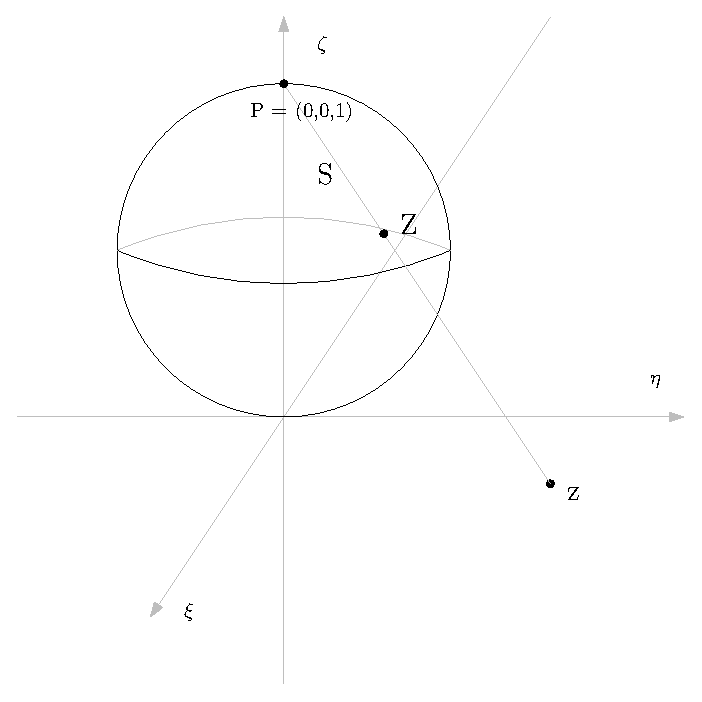
\includegraphics[scale=0.75]{Riemann.eps}
    \caption{Сфера Римана}
		\label{fig:2.1}
\end{figure}
\Def
\textbf{Стереографическая проекция:}
\begin{align*}
  & \forall z \in \CC \ \exists Z \in (\xi, \eta, \zeta): \ \left\{ \begin{matrix}
          \xi = tx \\
          \eta = ty \\
          \zeta = 1-t
      \end{matrix} \right., \ t \in [0;1]
\end{align*}
\begin{align*}
  & t = \frac{1}{1+ \left| z \right|^2}, \ \xi = \frac{x}{1+ \left| z \right|^2}, \ \eta = \frac{y}{1+ \left| z \right|^2}, \ \zeta = \frac{\left| z \right|^2}{1+ \left| z \right|^2}
\end{align*}
\begin{align*}
  & S \setminus P \leftrightarrow \CC, \ P \leftrightarrow \infty
\end{align*}
\textbf{Свойства}
\begin{enumerate}
    \item Любая пряая или окружность на комплексной плоскости переходит в
    окружность на сфере Римана.
    \item Если любые две кусочно гладкие кривые $\gamma_1$ и $\gamma_2$
    пересекаются под углом $\alpha$ на комплексной плоскости, то их образы
    $\tilde{\gamma}_1$, $\tilde{\gamma}_2$ будут пересекаться под тем же углом
    $\alpha$ на сфере Римана.
\end{enumerate}
\Def
$f: G \mapsto D$, где $G$~--- область, $D \subseteq \CCC$~--- область или вся
(расширенная) комплексная плоскость; $f(z) = u(x,y) + iv(x,y)$~---
\textbf{функция комплексного переменного.}
\Def
Пусть $z_0$~--- предельная точка $G \subseteq \CCC$ и $f: G \mapsto \CCC$; тогда
число $A$ назыается \textbf{пределом} $f$ в этой точке (пишется $\dst \lim_{z \to
  z_0} f(z_0)$) тогда и только тогда, когда выполняется
\begin{equation}\label{(2.3)}
    \forall \varepsilon > 0 \ \exists \delta(\varepsilon) > 0: \ z \in \os{\circ}{B}_\delta(z_0)\cap G \hookrightarrow f(z) \in B_\varepsilon (A)
\end{equation}
\asm
\begin{align*}
  & \exists \lim_{z \to z_0}f(z) = A = a+ib \Leftrightarrow \left\{ \begin{matrix}
          \dst \lim_{(x,y)\os{G}{\to}(x_0,y_0)}u(x,y) = a \\
          \dst \lim_{(x,y)\os{G}{\to}(x_0,y_0)}v(x,y) = b
      \end{matrix} \right.
\end{align*}
\pr
Очевидно по аналогии с последовательностями.
\Def
$f: G \mapsto \CCC$ \textbf{непрерывна} в $z_0 \in G \subseteq \CCC$, если
$z_0$~--- предельная точка $G$ и $\dst \lim_{z \to z_0} = f(z_0)$.
\asm
Функция непрерывна тогда и только тогда, кода ее действителная и мнимая части
непрерывны.
\pr Очевидно по аналогии с пределом.
\Def
\textbf{Функциональным рядом} называется сумма вида $\dst \sum_{n=1}^\infty
f_n(z)$, где $\forall n \in \NN \ f_n :G \mapsto \CC$.
\Def
Ряд \textbf{сходится равномерно}, если он:
\begin{enumerate}
    \item $\forall z \in G$ сходится к некоторой $S(z)$;
    \item $\forall \varepsilon > 0 \ \exists N(\varepsilon) > 0: \ \forall N \geq N
    (\varepsilon) \ \left| \dst \sum_{n=1}^Nf_n(z) - S(z) \right|\leq
    \varepsilon$.
\end{enumerate}
Все критерии и признаки для таких рядов аналогичны таковым в действительном
анализе.    
    \newpage
   	\setcounter{section}{9}
\section{Глава 10. Кратные интегралы}
\subsection{Определение кратного интеграла}
\subsubsection{Случай, когда $f(x)$ - ограниченная функция.}
\begin{Def}
Пусть $f$ -- ограниченная функция, заданная на измеримом по Лебегу Жордану) множестве $E \subset \R^n$ конечной меры. 

$\textbf{Разбиением}$ множества $E$ называется $E=\bigsqcup\limits_{k=1}^N E_k$, где $E_k$ - измеримые по Лебегу (Жордану). \newline В качестве $\Delta x_k$ будем брать меру множеств $E_k$. 

Обозначим $M_k=\sup\limits_{x\in E_k} f\left(x\right) ,\  m_k=\inf\limits_{x\in E_k}f\left(x\right)$ \newline
Суммы Дарбу - Лебега (Жордана): верхняя $\mathcal{U}(P, f)=\sum\limits_{k=1}^N M_k \cdot \mu_{(J)}(E_k)$, нижняя $L(P, f)\?=\sum\limits_{k=1}^N m_k \cdot \mu_{(J)}(E_k)$.
\newline Верхний интеграл Лебега или Римана (L)(R)$\ \overline{I}_E(f)=\inf\limits_P \mathcal{U}(P, f)$,\newline Нижний интеграл Лебега или Римана (L)(R)$\ \underline{I}_E(f)=\sup\limits_P L(P, f)$
\end{Def}
\begin{Def}
Если (R)$\ \overline{I}_E(f)=$ (R)$\ \underline{I}_E(f)$, то $f$ называется интегрируемой по Риману на $E$, $\int\limits_E f(x)dx=$ (R)$\ \overline{I}_E(f)$ \newline
Если (L)$\ \overline{I}_E(f)=$ (L)$\ \underline{I}_E(f)$, то $f$ называется интегрируемой по Лебегу на $E$, $\int\limits_E f(x)d\mu (x)\?= \text{(L) }\overline{I}_E(f)$
\end{Def}
\textbf{Утв. 1} Функция $f$ интегрируема по Риману на $[a,b]$(в смысле старого определения) $\Leftrightarrow$ $f$ интегрируема по Риману на $E=[a,b] \subset \R^1$.
\begin{proof}
$(\Rightarrow)$	Составим цепочку неравенств:
\begin{equation}
\underline{I}(f) \overset{(1)}{\leqslant} \text{(R) }\underline{I}_{[a,b]}(f)\overset{(2)}{\leqslant} \text{(L) }\underline{I}_{[a,b]}(f)\overset{(3)}{\leqslant}\text{(L) } \overline{I}_{[a,b]}(f) \overset{(4)}{\leqslant} \text{(R) } \overline{I}_{[a,b]}(f)\overset{(5)}{\leqslant} \overline{I}(f)\tag{10.1.1}\label{10.1.1} 
\end{equation}

Неравенство (1) следует из того, что в старом определении мы делили на отрезки, которые пересекаются в концах, а в новом определении идет разбиение на непересекающиеся, измеримые по Жордану множества.

Неравенство (2) следует из того, что нижние интегралы в смысле Римана и в смысле Лебега отличаются тем, на какие множества мы разбиваем: измеримые по Жордану или Лебегу. Но так как каждое измеримое по Жордану автоматически измеримо по Лебегу, то в $\text{(L) }\underline{I}_{[a,b]}(f)$ мы берем точную верхнюю грань по большему множеству.

Неравенства (4), (5) следуют из выше доказанных, но в обратном порядке.

Доказательство неравенства (3): хотим установить, что для любых двух разбиений $P_1, P_2\ L(P_1, f) \leqslant \mathcal{U}(P_2, f)$, что и докажет требуемое неравенство. Для этого необходимо взять общее измельчение разбиений $P=P_1 \bigcup P_2$ и получить цепочку неравенств $L(P_1, f) \leqslant L(P, f) \leqslant \mathcal{U}(P, f) \leqslant \mathcal{U}(P_2, f)$. Получим это: составим два произвольных разбиения 
$P_1 : E = \bigsqcup\limits_{k=1}^{N_1} E_k^{(1)},\ P_2 : E = \bigsqcup\limits_{k=1}^{N_2} E_k^{(2)}$. Тогда общее измельчение $ P : E = \bigsqcup\limits_{k=1}^{N_1} \bigsqcup\limits_{j=1}^{N_2} E_k^{(1)} \bigcap E_j^{(2)}$.
Докажем неравенство для нижних сумм:

 $L(P_1, f)=\sum\limits_{k=1}^{N_1} \inf\limits_{x\in E_k^{(1)}}f(x) \cdot \mu_{(J)}(E_k^{(1)}) =
\sum\limits_{k=1}^{N_1} \inf\limits_{x\in E_k^{(1)}}f(x) \sum\limits_{j=1}^{N_2} \mu_{(J)} (E_k^{(1)}\bigcap E_j^{(2)})\?\leqslant \sum\limits_{k=1}^{N_1}\sum\limits_{j=1}^{N_2}\inf\limits_{x\in E_k^{(1)}\bigcap (E_j^{(2)}}f(x)\cdot \mu_{(J)} (E_k^{(1)}\bigcap E_j^{(2)})=L(P,f)$, так как инфимум по $E_k^{(1)}$ не превосходит инфимум по $E_k^{(1)}\bigcap E_j^{(2)}$ для каждого $j$. Аналогично доказывается оставшаяся часть неравенства.

Из доказанного неравенства \ref{10.1.1} следует, что из интегрируемости по Риману в старом смысле, мы получили интегрируемость в новом смысле, так как $\underline{I}(f) = \overline{I}(f)$, а также, что из интегрируемости по Риману следует интегрируемость по Лебегу.

$(\Leftarrow$)
Отступление.
Вспомним критерий интегрируемости:
$$f\in R[a,b] \Leftrightarrow (\forall \varepsilon > 0)(\exists P)\ \mathcal{U}(P, f)-L(P, f)<\varepsilon$$
В доказательстве мы использовали тот факт, что $\overline{I}(f)=\inf\limits_P \mathcal{U}(P, f)$, $\ \underline{I}(f)=\sup\limits_P L(P, f)$, и так как $\mathcal{U}(P, f)-L(P, f)<\varepsilon$, то и $\overline{I}(f) - \underline{I}(f) < \varepsilon$. Эта разность всегда неотрицательная, меньше любого положительного числа, значит равна 0. Вместо интегрируемости по Риману на отрезке можем написать интегрируемость по Риману на любом измеримом по Жордану или Лебегу.

Вернемся к доказательству.

 Пусть функция интегрируема по Риману в новом смысле: $\exists \int\limits_{[a,b]}f(x)dx$, тогда по критерию интегрируемости: $(\forall \varepsilon > 0)(\exists P:[a,b]=\bigsqcup\limits_{k=1}^{N} E_k) \mathcal{U}(P,f)-L(P,f)<\varepsilon$, где $E_k$ - измеримые по Жордану множества. Внутренняя мера Жордана $\mu_{*}^J(E_k)=\sup\limits_{M \subset E_k} |M|$, где $M$ - элементарное множество. Элементарным множеством на прямой является объединение конечного числа промежутков. Тогда 
$$\exists\text{ набор точек } \{a_j^{(k)}, b_j^{(k)}\},\ \bigsqcup\limits_{j=1}^{n_k}[a_j^{(k)}, b_j^{(k)}] \subset E_k,\ \mu_jE_k \backslash \bigsqcup \limits_{j=1}^{n_k}[a_j^{(k)}, b_j^{(k)}]) < \dfrac{\varepsilon}{2\cdot C \cdot N},$$
\mbox{где $|f(x)|\leqslant C$. Возьмем разбиение в старом смысле $Q: a=x_0 < x_1 < \ldots < x_{\nu} = b,$} $\text{где множество точек }\{x_i\}_{i=1}^{\nu} = \{a_j^{(k)}, b_j^{(k)}\}_{j=1}^{n_k},  k=\overline{1,\ldots,N}$.
Оценим $\mathcal{U}(Q, f)-L(Q, f)=\sum\limits_{i=1}^{\nu}(\sup\limits_{[x_{i-1}, x_i]}f(x)-\inf\limits_{[x_{i-1}, x_i]}f(x))\cdot \Delta x_i = \sum\limits_{k=1}^N \sum\limits_{j=1}^{n_k}(\sup\limits_{x\in [a_j^{(k)},b_j^{(k)}]}f(x)-\inf\limits_{x\in [a_j^{(k)},b_j^{(k)}]}f(x) )(b_j-a_j )+\sum\limits_{x\in B}(\sup\limits_{[x_{i-1}, x_i]}f(x)-\inf\limits_{[x_{i-1}, x_i]}f(x))\Delta x_i \leqslant \sum\limits_{k=1}^N(M_k-m_k)\sum\limits_{j=1}^{n_k}(b_j-a_j)+\sum\limits_{i\in B}\ldots \leqslant \sum\limits_{k=1}^N (M_k-m_k)\cdot \mu_{J}(E_k)+2\cdot C\cdot \sum\limits_{i\in B}\Delta x_i < 2\varepsilon$
\end{proof}
.
\begin{wrapfigure}{r}{0.5\linewidth}
	\includegraphics[width=\linewidth]{images/1.png}
\end{wrapfigure}
\begin{Def}
	\mbox{Пусть $ f:E\to\mathbb{R} $} ---  ограниченная измеримая на измеримом по Лебегу множестве \mbox{$ E\subset\mathbb{R}^n $} конечной меры функция.

	Если $ M=\sup\limits_{x\in E}f(x), $ $ m=\inf\limits_{x\in E}f(x), $ то \textbf{разбиением Лебега}, отвечающим разбиению $ Q=\{m=y_0<y_1<\ldots <y_N=M\}, $ называется разбиение
	$ P: E=\bigsqcup\limits_{i=1}^{N}E_i$, \mbox{где $E_i=\{x\in E: fx)\in [y_{i-1}, y_i)\},$} $i=1, \ldots, N-1$.
	\newline
	$E_N= \{x\in E: fx)\in [y_{N-1}, y_N]\}$
	\newline
	\newline
	\mbox{Тогда интегральной суммой Лебега назовем $S(Q, f, \{t_i\})=\sum\limits_{i=1}^N f(t_i)\mu(E_i)$, где $t_i \in E_i,$}$ 
	\newline i = 1, \ldots, N$.
\end{Def} 
\begin{theorem}(Основная теорема об интеграле Лебега от ограниченных функций).
	Если $f(x)$ ограниченная измеримая на измеримом по Лебегу множестве $ E\subset\R^n $ конечной меры  функция, то она интегрируема по Лебегу (суммируема) на $E$, причем ее интеграл равен пределу интегральных сумм с разбиениями Лебега, отвечающими разбиениям  $ Q $, при стремящемся к нулю диаметре последнего, т.е. $$\int\limits_E f(x)d\mu(x)=\lim_{\Delta(Q)\to 0}S(Q,f,\{t_i\}).$$
	Это значит, что $(\forall \varepsilon >0)(\exists \delta > 0)(\forall Q, \Delta(Q)<\delta) \text{ и } \forall \{t_i\}, t_i \in E_i, i=1,\ldots, N,$ где $E=\bigsqcup\limits_{i=1}^N E_i$ --- разбиение Лебега, отвечающее разбиению $Q$ отрезка $[m, M]$, выполняется $|S(Q, f, \{t_i\})-\int\limits_E f(x)d\mu(x)|<\varepsilon$.
\end{theorem}

\begin{proof}
	Прежде всего заметим, что если $P: E=\bigsqcup\limits_{i=1}^N E_i$, то\newline $L(P, f)\leqslant S(Q, f, \{t_i\})\leqslant \mathcal{U}(P, f)$. Кроме того $\mathcal{U}(P, f) - L(P, f) = \sum\limits_{i=1}^N(M_i-m_i)\mu(E_i) \?\leqslant \sum\limits_{i=1}^N (y_i-y_{i-1})\cdot\mu(E_i)\leqslant \Delta(Q) \sum\limits_{i=1}^N\mu(E_i)=\Delta(Q)\mu(E)$. В качестве $\delta = \dfrac{\varepsilon}{\mu(E)}$. Для множеств $ E $ меры нуль утверждение очевидно, так как все суммы (верхние, нижние, интегральные) в этом случае равны нулю.
\end{proof}

\subsubsection{Случай, когда $f(x)\geqslant 0$.}
Пусть $f(x)\geqslant 0$ - измеримая на измеримом по Лебегу множестве $E$ конечной меры функция. В качестве разбиений будем допускать и разбиения на счетное число измеримых по Лебегу множеств: $E = \bigsqcup\limits_{i=0 }^{\infty}E_i,\ E_0:=\{x\in E:f(x)=+\infty\}$. Обратите внимание! Индексацию ведем с 0, и $E_0$ жестко фиксируем. Соглашение: если $\mu(E_0)=0$, то $(+\infty)\cdot \mu(E_0)=0$. Получаем, что мы ничего не можем сказать о $M$, а $m=0$. 

Тогда разбиение принимает вид $Q: 0=y_0<y_1<\ldots$. 

В качестве $E_i = \{x\in E: f(x)\in[y_{i-1}, y_i)\}, i=1,\ldots$.

$\Delta(Q):=\sup\limits_{i=1, \ldots}(y_i-y_{i-1})$, может равняться и $+\infty$.

$L(P, f)=\sum\limits_{i=0}^{\infty}m_i\cdot \mu(E_i),\  \mathcal{U}(P, f)=\sum\limits_{i=0}^{\infty}M_i\cdot \mu(E_i)$ 

\begin{theorem}Основная теорема об интеграле Лебега для неограниченных измеримых функций)
Если $f(x)$ - неотрицательная, измеримая на измеримом по Лебегу множестве $E\subset \R^n$ конечной меры, то она интегрируема по Лебегу на $E$, причем
$\int\limits_E f(x)d\mu(x)\?=\lim\limits_{\Delta(Q)\to0}S(Q, f, \{t_i\}).$ 

При конечном значении интеграла понятие предела такого вида -- то же, что и в предыдущей основной теореме, если же интеграл бесконечен, то требуется, чтобы \newline$(\forall \varepsilon>0)( \exists \delta > 0)(\forall Q, \Delta(Q)<\delta) \text{ и } \forall \{t_i\}, t_i \in E_i, i=1,\ldots$, где $E=\bigsqcup\limits_{i=1}^{\infty} E_i$ --- разбиение Лебега, отвечающее разбиению $Q$ полуоси $[0, +\infty)$, выполняется $S(Q, f, \{t_i\})\geqslant\varepsilon$.
\end{theorem}

\begin{proof}
В случае конечного интеграла, доказательство аналогично доказательству предыдущей теоремы. Если интеграл бесконечен, то и предел интегральных сумм бесконечность, так как все $S$ зажаты между $\mathcal{U}(P, f) \:\text{и} \:L(P, f)$.
\end{proof}

\begin{Def}
Если $\int\limits_E f(x)d\mu(x) < +\infty$, то $f$ называется суммируемой на $E$.
\end{Def}

\subsubsection{Случай, когда $f(x)$ - любого знака.}
Пусть $f(x)$ измерима на измеримом по Лебегу множестве $E \subset \R^n$ конечной меры. Введем $f_+(x):=\max(f(x), 0), f_-(x):=\max(-f(x), 0)$ - это неотрицательные, измеримые функции. Такие функции интегрируемы по Лебегу, то есть существуют $\int\limits_E f_+(x)d\mu(x), \int\limits_E f_-(x)d\mu(x)$. Если хотя бы один из этих интегралов конечен, то $f$ называется интегрируемой по Лебегу. Если оба конечны, то $f$ - суммируемая на $E$.
$$\int\limits_E f_+(x)d\mu(x)- \int\limits_E f_-(x)d\mu(x) = \int\limits_E f(x)d\mu(x)$$
Пример измеримой, но не интегрируемой по Лебегу функции: возьмем отрезок, на одной его половине функция равна $+\infty$, на другой $-\infty$.



   	\newpage
   	\section{Лекция 3. Недетерминированные конечные автоматы.}

Вспомним формальное определение (\ref{eq:FA}) конечного автомата.

\textbf{\text{Конечный автомат }} $\mathcal{A}$ --- устройство, описываемое набором $\langle Q$, $\Sigma$, $q_0$, $\delta$, $F \rangle$:
\begin{enumerate}
  \item {\bfseries\itshape{Q}} - конечное множество состояний автомата;
  \item $\boldsymbol{\Sigma}$ - алфавит, слова над которым обрабатывает автомат;
  \item $\boldsymbol{q_0}$ - начальное состояние автомата;
  \item $\boldsymbol{\delta}$ : $Q \times (\Sigma\cup\{\varepsilon\} ) \rightarrow 2^{Q}$ - функция переходов
  \item $\boldsymbol{F} \subset \boldsymbol{Q}$ - множество принимающих состояний.
\end{enumerate}


\begin{wrapfigure}{r}{0.3\textwidth}
  \centering
  \begin{tikzpicture}[node distance=2cm,on grid,auto]
    \node[state,initial] (q_0)   {$q_0$};
    \node[state,accepting] (q_1) [right=of q_0] {$q_1$};
    \path[->]
    (q_0) edge [bend left] node {$b$} (q_1)
    (q_0) edge [loop above] node {$a,b$} ()
    (q_1) edge [bend left] node {$\varepsilon$} (q_0);
  \end{tikzpicture}
  \caption{Пример НДА.}
  \label{fig:NFAexample}
\end{wrapfigure}

Рассмотрим рисунок (\ref{fig:NFAexample}). К примеру сразу из определения и графа имеем: $\delta(q_0,\:b)=\{q_0,q_1\}$.

\begin{question}
  Неформально опишите язык, распознаваемый данным автоматом.
\end{question}

\begin{nonum}
  Язык $R$, состоящий из слов, оканчивающихся на $b$.

  В самом деле, в принимающее состояние можно перейти по единственному переходу на котором написан символ $b$, то есть $L(\mathcal{A})\subseteq R$.
  Далее любое слово, оканчивающееся на $b$ принимается автоматом, потому что, обрабатывая все символы слова автомат может оставаться в состояний
  $q_0$, а когда встретится последний символ(он же буква $b$) перейти в состояние $q_1$. Итак, $R\subseteq L(\mathcal{A})$.
\end{nonum}

\subsection{Алгоритм проверки принадлежности слова языку, распознаваемому НКА.} \label{alg:word}

В случае ДКА все тривиально. Просто эмулируем работу автомата на входном слове. Каждое следующее состояние определяется однозначно.
Обработав слово за линейное время выясняем принимается ли оно автоматом.

В случае НКА может быть несколько путей вычесления, к примеру для слова $bb$ в автомате на рисунке (\ref{fig:NFAexample})
есть более одного пути: $$q_0\xrightarrow{b} q_0\xrightarrow{b} q_1,$$
$$q_0\xrightarrow{b} q_1\xrightarrow{\varepsilon} q_0\xrightarrow{b} q_0.$$

Заметим, что не обязательно все возможные пути заканчиваются в принимающем(или не принимающем) состоянии, в приведенном примере один путь
заканчивается, другой --- нет.

\paragraph*{Алгоритм.} Пусть есть слово $w = w_1w_2\ldots w_n$, $w_i\in\Sigma^*$. На $i$"=ом шаге будем помнить и пересчитывать множество состояний
$Q_i=\{q\:|\:q_0\xrightarrow{w[1,i]}q\}$.

Итак, если после обработки слова, в $Q_n$ есть принимающее состояние, то слово принимается.
Для более формального описания алгоритма, введем функцию
$$\varepsilon\text{-closure}(S)=S\cup \{q\:|\:\exists p\in S\: :\: p\xrightarrow{\varepsilon}q\}$$

Наконец, опишем алгоритм формально:

\begin{enumerate}
  \item Построить множество $Q_0$ = $\varepsilon$"=closure($q_0$).
  \item Для $k$ от 1 до $|w|$ построить множества:
        \begin{itemize}
          \item $Q_k'=\{p\:|\:\exists q\in Q_k\: :\: p\in\delta(q,\:w_k)\}$;
          \item $Q_{k+1}=\varepsilon\text{-closure}(Q_k')=\displaystyle{\bigcup _{q'\in Q_k'}}\varepsilon\text{-closure}(q')$;
        \end{itemize}
  \item Если $Q_{|w|}\cap F_{\mathcal{A}}\neq \varnothing$, то ответ <<Да>>, иначе <<Нет>>.
\end{enumerate}


\begin{question}
  Как эффективно вычислить $\varepsilon\text{-closure}(S)$?
\end{question}

\begin{nonum}
  Рассмотрим подграф графа автомата, в котором оставлены только ребра, на которых написано $\varepsilon$.
  И дальше для каждого состояния из $S$ обходом в глубину(или в ширину) будем искать все достижимые состояния.
\end{nonum}


\subsection{Построение НКА по РВ.}

Напомним, что по определению любой регулярный язык
можно построить согласно следующей схеме:

\begin{enumerate}
  \item $\varnothing \in REG$
  \item $\forall\sigma \in \sum \implies \{\sigma\} \in  REG$
  \item $\forall X, Y \in REG: X \circ Y, X|Y, X^* \in REG$
\end{enumerate}

Мы будем строить НКА по РВ для каждого пункта. Более того,
нам потребуется соблюсти технические условия:

\begin{enumerate}[(i)]
  \item НКА имеет ровно одно принимающее состояние;
  \item В начальное состояние НКА не ведёт ни один переход;
  \item Из принимающего состояния НКА нет ни одного перехода.
\end{enumerate}

\begin{question}
  Построить такой автомат для
  \begin{itemize}
    \item Пустого языка;
    \item Языка, состоящего из одного символа.
  \end{itemize}
\end{question}


\begin{nonum}
  Приведем только ответы, корректность очевидна.

  \begin{figure}[!h]
    \centering
    \begin{minipage}{.5\textwidth}
      \centering
      \begin{tikzpicture}[node distance=2cm,on grid,auto]
        \node[state,initial] (q_0)   {$q_0$};
        \node[state,accepting] (q_1) [right=of q_0] {$q_1$};
      \end{tikzpicture}
      \caption{Пустой язык.}
    \end{minipage}%
    \begin{minipage}{.5\textwidth}
      \centering
      \begin{tikzpicture}[node distance=2cm,on grid,auto]
        \node[state,initial] (q_0)   {$q_0$};
        \node[state,accepting] (q_1) [right=of q_0] {$q_1$};
        \path[->]
        (q_0) edge node {$a$} (q_1);
      \end{tikzpicture}
      \caption{Язык $\{a\}$.}
    \end{minipage}
  \end{figure}
\end{nonum}


Осталось построить автоматы для пункта (3) определения регулярного языка. Будем изображать НКА схематично, помечая в них только начальное и принимающее состояния:
\begin{figure}[!h]
  \centering
  \begin{tikzpicture}[node distance=2cm,on grid,auto]
    \draw (0.5,0) ellipse (3cm and 1.5cm);
    \node[state,initial] (q_0)   {$q_0$};
    \node[] at (1,0) {$\mathcal{A}$};
    \node[state,accepting] (q_1) [right=of q_0] {$q_1$};
  \end{tikzpicture}
  \caption{Автомат, удовлетворяющий условиям (i–iii).}
\end{figure}

Далее, мы будем предполагать, что начальное состояние на схеме
находится слева, а принимающее справа.
Допустим уже построены автоматы $\mathcal{A}$ и $\mathcal{B}$ (удовлетворяющие условиям (i–iii)) для регулярных языков
$X$ и $Y$ соответственно. Построим
явно автомат, распознающий $X \cdot Y$.

\begin{figure}[!ht]
  \centering
  \begin{tikzpicture}[node distance=4.5cm,on grid,auto,initial text=]
    \draw (1,0) ellipse (2cm and 1cm);
    \draw (3.5,0) ellipse (2cm and 1cm);
    \draw (2.25, 0) circle (0.5cm);
    \node[state,initial] (q_0)   {$q_0^{\mathcal{A}}$};
    \node[state,accepting] (q_1) [right=of q_0] {$q_F^{\mathcal{B}}$};
    \node[] at (1,0) {$\mathcal{A}$};
    \node[] at (3.5,0) {$\mathcal{B}$};
  \end{tikzpicture}
  \caption{Автомат для конкатенации.}
  \label{fig:concatFA}
\end{figure}

Как видно из рисунка \ref{fig:concatFA}, результирующий автомат получен из автоматов $\mathcal{A}$ и $\mathcal{B}$
следующим образом. Начальное состояние автомата $\mathcal{B}$
\textit{склеено} с начальным состоянием автомата $\mathcal{A}$:
мы удалили из автомата $\mathcal{B}$ начальное состояние $q_0^{\mathcal{B}}$, а все переходы, которые вели из него,
добавили к принимающему состоянию $q_F^{\mathcal{A}}$
автомата $\mathcal{A}$, которое сделали непринимающим.
Дабы определить склейку состояний для произвольных автоматов, скажем, что если бы в состояние $q_0^{\mathcal{B}}$ вели какие-то
переходы, то их бы также направили в состояние, полученное в результате склейки.


Далее строим автомат для языка $X | Y$ используя конструкцию:

\begin{figure}[!ht]
  \centering
  \begin{tikzpicture}[node distance=3cm,on grid,auto,initial text=]
    \node[state,initial] (q_0)   {$q_0$};
    \node[state] (q_0a) [above right=of q_0] {$q_0^{\mathcal{A}}$};
    \node[state] (q_fa) [right=of q_0a] {$q_F^{\mathcal{A}}$};
    \node[state] (q_f) [below right=of q_fa] {$q_F$};
    \node[state] (q_0b) [below right=of q_0] {$q_0^{\mathcal{B}}$};
    \node[state] (q_fb) [right=of q_0b] {$q_F^{\mathcal{B}}$};
    \node[] at (3.6, 2.1) {$\mathcal{A}$};
    \node[] at (3.6, -2.1) {$\mathcal{B}$};
    \draw (3.6, 2.1) ellipse (2.5cm and 1cm);
    \draw (3.6, -2.1) ellipse (2.5cm and 1cm);
    \path[->]
    (q_0) edge node {$\varepsilon$} (q_0a)
    (q_0) edge node {$\varepsilon$} (q_0b)
    (q_fa) edge node {$\varepsilon$} (q_f)
    (q_fb) edge node {$\varepsilon$} (q_f);
  \end{tikzpicture}
  \caption{Автомат для конкатенации.}
  \label{fig:sumFA}
\end{figure}


И наконец перейдём к построению автомата для языка $X^*$:


\begin{figure}[!ht]
  \centering
  \begin{tikzpicture}[node distance=2.5cm,on grid,auto,initial text=]
    \node[state,initial] (q_0)   {$q_0$};
    \node[state] (q_0a) [right=of q_0] {$q_0^{\mathcal{A}}$};
    \node[state] (q_fa) [right=of q_0a] {$q_F^{\mathcal{A}}$};
    \node[state] (q_f) [right=of q_fa] {$q_F$};
    \draw (3.75,0) ellipse (2cm and 1cm);
    \node[] at (3.75,-0.5) {$\mathcal{A}$};
    \path[->]
    (q_0) edge node {$\varepsilon$} (q_0a)
    (q_0) edge [bend left] node {$\varepsilon$} (q_f)
    (q_fa) edge [bend right] node {$\varepsilon$} (q_0a)
    (q_fa) edge node {$\varepsilon$} (q_f);
  \end{tikzpicture}
  \caption{Автомат $C$ для итерации.}
  \label{fig:iterFA}
\end{figure}


\begin{proof}

  По индукции докажем, что для $\forall n>0$ $w\in X^n\Rightarrow w\in L(C)$, то есть докажем включение $X^*\subseteq L(C)$.

  \underline{База}: пустое слово принимается автоматом.

  \underline{Переход}: Рассмотрим слово $w=u_1\cdot u_2\cdot\ldots\cdot u_n$, $u_i\in L(\mathcal{A})$. Слово
  $v=u_1\cdot u_2\cdot\ldots\cdot u_{n-1}\in L(C)$ по предположению индукции. Есть несколько вариантов.
  \begin{itemize}
    \item $v$ --- пустое. Но тогда можно попасть в состояние $q_0^{\mathcal{A}}$, а из него, так как $u_n$ принимается $\mathcal{A}$,
          в состояние $q_F^{\mathcal{A}}$, откуда уже в $q_F$.
    \item $v$ --- непустое. Это означает, что путь по нему из начального состояния в принимающее обязательно прошел через
          $q_F^{\mathcal{A}}$. Тогда вернемся на шаг назад в состояние $q_F^{\mathcal{A}}$, а из него еще на шаг в состояние
          $q_0^{\mathcal{A}}$ по ребру $\varepsilon$. И оттуда уже обрабатываем слово $u_n$.
  \end{itemize}

  Теперь докажем $L(C)\subseteq X^*$.

  Пусть слово $w\in L(c)$. Если $w$ --- пустое, то оно очевидно принадлежит $X^*$. Если же слово не пустое, посмотрим на путь из $q_0$.
  Если этот путь не проходил через ребро $q_F^{\mathcal{A}}\xrightarrow{\varepsilon} q_0^{\mathcal{A}}$, тогда все очевидно.

  Если же этот переход был, найдем первый этот переход, который случился после того, как был обработан какой-то непустой префикс слова $w$.
  Заметим, что этот префикс есть собственный префикс $w$ и по предположению индукции этот префикс принадлежит $X^*$. Заметим, что и суффикс принадлежит
  $X^*$, но тогда и $w$ принадлежит $X^*$.

\end{proof}


\subsection{Построение ДКА по НКА.}

Модифицируем алгоритм проверки принадлежности слова языку, распознаваемому НКА. Заметим, что число множеств $Q_k$,
появлявшихся в алгоритме, конечно, поскольку $Q_k \subseteq 2^{Q_{\mathcal{A}}}$. Поэтому всевозможные множества
можно хранить в конечной памяти, они и будут состояниями ДКА, который мы назовём $2^{\mathcal{A}}$.
Начальным состоянием будет состояние $Q_0$,
принимающими будут множества $Q_k$, содержащие принимающие состояния $\mathcal{A}$, а переходы между состояниями определены, как и в алгоритме:

\begin{enumerate}
  \item $Q_0 = \varepsilon\text{-closure}(q_0)$
  \item $\delta (Q', a)=\varepsilon\text{-closure}(\widetilde{Q}')$, где
        $\widetilde{Q}'=\{q\:|\: \exists p\in Q':\:p\in\delta(p, a)\}=\displaystyle{\bigcup_{p\in Q'}}\delta(p, a).$
\end{enumerate}


\subsection{Построение РВ по НКА.}

\begin{Def}
  \textit{Обобщенный НКА} --- НКА, у которого вместо букв на переходах написаны регулярные выражения.

  Слово $w\in L(\mathcal{A})$, если существует разбиение $w=u_1\cdot u_2\cdot\ldots\cdot u_n$, $u_i\in \Sigma^*$ и существует
  последовательность состояний $q_1, q_2, \ldots, q_n\in F$, такие что $u_1\in R_{q_0, q_1}$, $u_2\in R_{q_1, q_2}$, \ldots, $u_n\in R_{q_{n-1}, q_n}$, где
  $R_{q_i,q_j}$ --- РВ написанное на ребре $q_i\rightarrow q_j$.
\end{Def}

Основная идея такая. Вначале нужно превратить НКА в НКА с одним принимающем состоянием, в который не ведет ни одно ребро и с начальным состоянием
в которое также ничего не ведет (рисунок (\ref{fig:prepare})).

\begin{figure}
  \centering
  \begin{tikzpicture}[node distance=3cm,on grid,auto,initial text=]
    \node[state,initial] (q0)   {$q_0$};
    \node[state, initial] (q1) at (1,3) {};
    \node[state,accepting] (p) at (5, 0) {$p$};
    \node[state,accepting] (r1) at (4.5, 2.5) {};
    \node[state,accepting] (r2) at (3, 2) {};
    \node[state,accepting] (r3) at (5, 4) {};
    \draw (3,3) ellipse (4cm and 2cm);
    \path[->]
    (q0) edge node {$\varepsilon$} (q1)
    (r1) edge node {$\varepsilon$} (p)
    (r2) edge node {$\varepsilon$} (p)
    (r3) edge [bend left, out=30, in=120] node {$\varepsilon$} (p);
  \end{tikzpicture}
  \caption{Начальная подготовка графа.}
  \label{fig:prepare}
\end{figure}


Далее делаем старые принимающие состояние непринимающими и переходим к следующему шагу.

Берем НКА и последовательно удаляем состояния, пересчитывая ребра.

\begin{wrapfigure}{r}{0.45\textwidth}
  \centering
  \begin{tikzpicture}[node distance=2.5cm,on grid,auto,initial text=]
    \node[state,initial] (q)   {$q$};
    \node[state] (p) [right=of q] {$p$};
    \node[state] (r) [right=of p] {$r$};
    \path[->]
    (q) edge node {$R_{q,p}$} (p)
    (p) edge node {$R_{p,r}$} (r)
    (p) edge [loop above] node {$R_{p,p}$} ()
    (q) edge [bend right, in=240] node {$R_{q,r}$} (r);
  \end{tikzpicture}
  \caption{Удаление состояния.}
  \label{fig:deleteNode}
\end{wrapfigure}


Допустим нужно удалить состояние $p$. Нужно рассмотреть все пары $(q, r)$ удовлетворяющие
рисунку (\ref{fig:deleteNode}).
Тогда после удаления $p$ нужно убрать все ребра на рисунке и добавить ребро $q\xrightarrow{R'_{q, r}}r$, где $$R'_{q,r}=R_{q,r}\cup R_{q,p}R^*_{p,p}R_{p,r}$$.

   	\begin{flushright}
    \textit{Лекция 4 (от 15.09)}
\end{flushright}

\textbf{Кривая} $\gamma$~--- класс эквивалентных параметризаций $z(t) = x(t) +
iy(t), \ t \in \left[ t_0; t_1 \right]$
\\
\textbf{Параметризации эквивалентны}, если существует монотонная возрастающая
функция $\psi(\tau) = t$, сохраняющая направление.
\\
\textbf{Гладкая кривая (ГК)}~--- такая кривая $\gamma$, что существует параметризация
$z(t) = x(t) + iy(t)$, $x \in C^1 \left( \left[ t_0; t_1 \right] \right)$, $y
\in C^1 \left( \left[ t_0; t_1 \right] \right)$, $\forall t \in \left[ t_0; t_1
\right] \ z'(t) \neq 0$.
\\
\textbf{Замкнутая ГК (ЗГК)}~--- такая ГК, что $z(t_0) = z(t_1)$, $z'(t_0+0) =
z'(t_1-0)$.
\\
\textbf{Кусочно гладкая кривая (КГК)}~--- такая непрерывная кривая $\gamma$, что
$\exists t_0 = \theta_0 < \theta_1 < \dots < \theta_{n-1} < \theta_n = t_1$, что
$\forall k \ \gamma_k: \ z(t), \ t \in [\theta_{k-1}, \theta_k]$ есть ГК.
\\
\textbf{Разбиение} отрезка $\left[ t_0, t_1 \right]$: $\lambda = \{t_0 = \tau_0
< \tau_1 < \dots < \tau_{m_\lambda} = t_1\}$.
\\
\textbf{Мелкость (диаметр)} разбиения $\lambda$ $\left| \lambda \right| = \dst
\max_{k \{1, \dots, m_\lambda\}}\left| \tau_k - \tau_{k-1} \right|$.
\Def Пусть $f: \gamma \mapsto \CC$ непрерывна на КГК $\gamma$. Пусть
$\lambda$~--- разбиение $\left[ t_0, t_1 \right]$ для $\gamma: \ z(t)$~---
кусочно гладкой. Пусть $z(t_k) = z_k, \ k \in \{0, \dots, m_\lambda\}$, $\zeta_k
\in \gamma_k = \gamma_{z_{k-1}z_k}$
\begin{align*}
  & \sigma(\lambda) = \sum_{k = 1}^{m_{\lambda}} f(\zeta_k) \Delta z_k
\end{align*}
$\Delta z_k = z_k - z_{k-1}$~--- \textbf{интегральная сумма};
\\
если $\exists \lim \sigma(\lambda) \ \forall \zeta_k, \ \left| \lambda \right|
\to 0$, то этот предел называется \textbf{интегралом Римана от $f$ по $\gamma$}
и записывается как
\begin{equation} \label{(6.1)}
    \int_{\gamma}f(z) dz
\end{equation}
\theorem
Если условия определения интеграла выполняются, то он существует и справедливо:
\begin{equation} \label{(6.2)}
    \int_{\gamma}f(z)dz = \int_{\gamma}\left( u dx - v dy \right) + i \int_\gamma \left( v dx + u dy \right)
\end{equation}
\pr
\begin{align*}
  & \sigma(\lambda) = \sum_{k = 1}^{m_\lambda}\left( u(\xi_k, \eta_k) + iv(\xi_k, \eta_k) \right)\left( \Delta x_k + i \Delta y_k \right) = \sum_{k = 1}^{m_\lambda}\left( u(\xi_k, \eta_k) \Delta x_k - v(\xi_k, \eta_k) \Delta y_k\right) + \\
  & + \left( v(\xi_k, \eta_k) \Delta x_k + u(x_k, y_k) \Delta y_k\right) = \sigma_1(\lambda) + \sigma_2(\lambda) \to \int_{\gamma}\left( u dx - v dy \right) + i \int_\gamma \left( v dx + u dy \right)
\end{align*}
\corollary
Если условия определения интеграла выполняются, то верно:
\begin{equation} \label{(6.3)}
    \int_\gamma f(z) dz = \int_{t_0}^{t_1}f(z(t))z'(t)dt
\end{equation}
\begin{equation} \label{(6.4)}
    \gamma: z(t), \ \int_{t_0}^{t_1}\left( P(t) + iQ(t) \right) dt = \int_{t_0}^{t_1}P(t)dt + i \int_{t_0}^{t_1}Q(t)dt
\end{equation}
\pr
Из \eqref{(6.2)} и свойств криволинейных интегралов II рода
\begin{align*}
  &\int_{\gamma}P(x,y) dx + Q(x,y)dy = \int_{t_0}^{t_1} \left( P(x(t), y(t))x'(t) + Q(x(t), y(t))y'(t) \right) dt
\end{align*}
\underline{\textbf{Общие свойства интеграла}}
\begin{enumerate}
    \item Линейность:
    \begin{align*}
      &\int_{\gamma}\left(\lambda f(z) + \mu g(z)\right) dz = \lambda\int_{\gamma}f(z) dz + \mu \int_\gamma g(z) dz
    \end{align*}
    \item Аддитивность вдоль кривой: если $\gamma = \gamma_1 \cup \gamma_2$
    (общая точка~--- только конец), то
    \begin{align*}
      &\int_{\gamma}f(z) dz = \int_{\gamma_1}f(z) dz + \int_{\gamma_2} f(z) dz
    \end{align*}
    \item Изменение знака при смене направления: если $\gamma^{-1}$~---
    кривая, совпадающая во всех точках с $\gamma$, но противоположно
    направленная, то
    \begin{align*}
      &\int_{\gamma^{-1}}f(z) dz = - \int_{\gamma}f(z) dz
    \end{align*}
    \item Инвариантность относительно замены параметра.
    \item Выполняется неравенство:
    \begin{equation} \label{(6.5)}
        \left| \int_\gamma f(z) dz \right| \leq \int_{\gamma}\left| f(z) \right| \cdot \left| dt \right| = \int_{t_0}^{t_1} \left| f(z(t)) \right| \sqrt{(x'(t))^2 + (y'(t))^2}dt
    \end{equation}
    \pr
    Из \eqref{(6.3)}:
    \begin{equation} \label{(6.6)}
        \left| \sigma(\lambda) \right| \leq \sum_{k = 1}^{m_\lambda}\left| f(\zeta) \right| \cdot \left| \Delta z_k \right|
    \end{equation}
\end{enumerate}
\example
\begin{align*}
  &J_k = \int_{\gamma: \left| z-a \right| = r} (z-a)^k dz, \ k \in \ZZ
\end{align*}
Параметр: $z(t)= a+re^{it}, \ t \in [0;2\pi]$
\begin{align*}
  & dz(t) = rie^{it}dt
\end{align*}
\begin{align*}
  &J_k = \int_{0}^{2\pi} r^ke^{ikt}rie^{it}dt = r^{k+1}i\int_{0}^{2\pi}e^{i(k+1)t} dt
\end{align*}
\begin{align*}
  &J_{-1} = 2 \pi i
\end{align*}
\begin{align*}
  &J_k = r^{k+1}i\int_{0}^{2\pi} \left( \cos(k+1)t + i \sin(k+1)t \right) dt = 0, \ k \neq -1
\end{align*}
\example
\begin{align*}
  &J_1 = \int_{\gamma} dz, \ J_2 = \int_{\gamma}z dz
\end{align*}
$\gamma: z(t)$, и согласно \eqref{(6.3)}
\begin{align*}
  &J_1 = \int_{t_0}^{t_1} z'(t)dt = z(t_1) - z(t_0)
\end{align*}
\begin{align*}
  &J_2 = \int_{t_0}^{t_1} z(t)z'(t)dt = \frac{1}{2}\int_{t_0}^{t_1}\frac{d}{dt}\left( z^2(t) \right)dt = \frac{1}{2}\left( z^2(t_1) - z^2(t_0) \right)
\end{align*}
\theorem
Пусть $f_n: G \mapsto \CC$ непрерывна на $G$ $\forall n \in \NN$, $\gamma$~---
КГК, $\gamma \subseteq G$.
\\
Пусть $\dst \sum_{n=1}^{\infty}f_n(z) \underset{\gamma}{\rightrightarrows} S(z)
\ \forall z \in \gamma$.
Тогда $S(z)$ непрерывна на $\gamma$ и выполняется
\begin{equation} \label{(6.7)}
    \int_{\gamma}S(z) dz = \sum_{n=1}^{\infty}\int_{\gamma}f_n(z)dz
\end{equation}
\pr
Ряд сходится равномерно на $\gamma$
\begin{align*}
  & \Updownarrow
\end{align*}
\begin{equation} \label{(6.8)}
    \forall \varepsilon > 0 \ \exists N(\varepsilon): \ \forall N\geq N(\varepsilon) \ \underset{z \in \gamma}{\sup} \left| S(z) - \sum_{n = 1}^{N}f_n(z) \right| = \underset{z \in \gamma}{\sup} \abs{S - S_N(z)} \leq \varepsilon
\end{equation}
\begin{align*}
  &\exists \delta > 0: \ \forall z_0 \in \gamma, \ z \in \gamma, \ \left| z - z_0 \right| < \delta: \ \left| S(z) - S(z_0) \right| \leq \left| S(z) - S_N(z) \right| +  \left| S_N(z) - \right. \\
  &\left. - S_N(z_0) \right| + \left| S_N(z_0) - S(z_0) \right| \leq \left| S_N(z) - S_N(z_0) \right| + 2 \varepsilon \leq 3 \varepsilon
\end{align*}
\begin{align*}
  & \Downarrow
\end{align*}
\begin{align*}
  & S(z) \rightarrow S(z_0)
\end{align*}
\begin{align*}
  & \Downarrow
\end{align*}
\begin{align*}
  & \exists \int_{\gamma}S(z)dz
\end{align*}
\begin{align*}
  &\forall N \geq N(\varepsilon) \ \left| \int_{\gamma}S(z)dz - \int_{\gamma}S_N(z)dz\right| = \left| \int_\gamma \left( S(z) - S_N(z) \right)dz\right| \leq \int_\gamma \left| S(z) - S_N(z) \right| \left| dz \right| \leq \\
  & \leq \varepsilon \int_{\gamma} \left| dz \right| = \varepsilon l(\gamma) = \varepsilon \cdot const
\end{align*}
Теорема доказана.
\Def
Пусть $g: G \mapsto \CC$ на области $G$; назовем это \textbf{первообразной}
непрерывной функции $f: G \mapsto \CC$, если $g$ регулярна на $G$ и $g'(z) =
f(z) \ \forall z \in G$.
\Def
Выражение $f(z)dz$ называется \textbf{полным дифференциалом в области $G$}, если
существует первообразная $g$ для $f$ на $G$, т.~е. $f(z)dz = g'(z)dz$.
\theorem
Пусть $f:G \mapsto \CC$ непрерывна на области $G$. Тогда:
\begin{enumerate}
    \item если $f dz$~--- полный дифференциал на $G$, то для любой замкнутой КГК
    $\overset{\circ}{\gamma} \subseteq G$ выполняется
    \begin{equation} \label{(6.9)}
        \int_{\overset{\circ}{\gamma}} f(z) dz = 0
    \end{equation}
    \item если для любой замкнутой ломаной кривой $\gamma$ выполняется
    \eqref{(6.9)}, то $f dz$~--- полный дифференциал.
\end{enumerate}
\pr ~
\\
\begin{enumerate}
    \item $\exists g:G \mapsto \CC$, регулярная, такая, что $g'(z) = f(z)$.
    Тогда
    \begin{align*}
      & \int_{\overset{\circ}{\gamma}} f(z) dz \underset{\overset{\circ}{\gamma}: z = z(t)}{=} \int_{t_0}^{t_1} g'(z(t))z'(t)dt = \int_{t_0}^{t_1}\frac{d}{dt}(g(z(t)))dt = g(z(t_1)) - g(z(t_0)) = \\
      & = g(z(t_1)) - g(z(t_1)) = 0
    \end{align*}
    \item Фиксируем $a \in G$ как начальную точку ломаной $\gamma$. $\forall z
    \in G$ $\exists \gamma_{az}$~--- ломаная с началом в $a$ и концом в $z$.
    \begin{align*}
      & g(z) = \int_{\gamma_{az}} f(z) dz
    \end{align*}
    не зависит от $\gamma_{az}$, а лишь зависит от $z$. Действительно, если
    $\exists \gamma_{az}, \ \exists \tilde{\gamma_{az}}$, то пусть
    $\overset{\circ}{\gamma} = \gamma_{az} \cup \tilde{\gamma_{az}}^{-1}$,
    тогда из \eqref{(6.8)}
    \begin{align*}
      & \int_{\overset{\circ}{\gamma}} f(z) dz = 0 = \int_{\gamma_{az}}f dz - \int_{\tilde{\gamma_{az}}}f(z)dz
    \end{align*}
    Докажем, что $\forall z \ g'(z) = f(z)$. Рассмотрим $z_0$; $\exists
    \varepsilon > 0: B_{\varepsilon}(z_0) \subseteq G$, $\Delta z: 0 <
    \left| \Delta z \right| < \varepsilon$. Тогда $z_0 + \Delta z \in G$.
    Рассмотрим
    \begin{align*}
      & \frac{g(z_0+\Delta z) - g(z_0)}{\Delta z}
    \end{align*}
    Тогда
    \begin{align*}
      & g(z+ \Delta z) = \int_{\gamma_{az_0} \cap [z_0; \Delta z + z_0]}
    \end{align*}
    \begin{align*}
      & \Downarrow
    \end{align*}
    \begin{align*}
      & \frac{g(z_0+ \Delta z) - g(z_0)}{\Delta z} = \frac{1}{\Delta z} \int_{[z_0; \Delta z + z_0]} f(z)dz
    \end{align*}
    \begin{align*}
      & \left| \frac{\Delta g}{\Delta z} - f(z_0) \right| = \left| \frac{1}{\Delta z} \int_{[z_0; \Delta z + z_0]}(f(z) - f(z_0))dz \right|
    \end{align*}
    В силу непрерывности $f(z)$, полагая $r(\varepsilon)$~--- радиус шара, где
    $\left| f(z) - f(z_0) \right| < \varepsilon$,
    \begin{align*}
      & \forall z \in B_{r(\varepsilon)}(z_0)\cap B_\varepsilon(z_0) \ \left| \frac{\Delta g}{\Delta z} - f(z_0) \right| \leq \left| \frac{\varepsilon\min\left\{ r(\varepsilon), \varepsilon \right\}}{\min\left\{ r(\varepsilon), \varepsilon \right\}} \right| = \varepsilon
    \end{align*}
\end{enumerate}

   	\begin{proof}
	Имеем множество $E$ необязательно конечной меры, $E=\bigsqcup\limits_{k=1}^\infty E_k$, $E_k$ --- измеримые по Лебегу множества, дополнительно предположим, что $f(x)\geqslant 0$. Хотим установить равенство $\int\limits_{E}f(x)d\mu(x)=\sum\limits_{k=1}^\infty \int\limits_{E_k}f(x)d\mu(x)$.
	
	Возьмем исчерпывание множествами конечной меры $E^{(1)}\subset E^{(2)}\subset \ldots,$ такими, что $\lim\limits_{s\to\infty}E^{(s)}=\bigcup\limits_{s=1}^\infty E^{(s)}=E$. Тогда по определению
	$$\int\limits_{E}f(x)d\mu(x)=\lim\limits_{s\to\infty}\int\limits_{E^{(s)}}f(x)d\mu(x).$$ Обозначим $a_k^{(s)}:=\int\limits_{E_k\cap E^{(s)}}f(x)d\mu(x)$. Заметим, что $E_k\cap E^{(s)}$ имеет конечную меру и $E_k\cap E^{(1)} \subset E_k\cap E^{(2)}\subset\ldots$, $\bigcup\limits_{s=1}^\infty \left( E_k\cap E^{(s)}\right) = E_k$, тогда $a_k:=\int\limits_{E_k}f(x)d\mu(x)=\lim\limits_{s\to\infty}\int\limits_{E_k\cap E^{(s)}}f(x)d\mu(x)=\lim\limits_{s\to\infty}a_k^{(s)}$.
	Все $a_k^{(s)}$ --- неотрицательные числа, значит по Лемме 10.3.1 имеет место равенство: $\lim\limits_{s\to\infty}\sum\limits_{k=1}^\infty a_k^{(s)}=\sum\limits_{k=1}^\infty a_k$. Получаем $\lim\limits_{s\to\infty}\sum\limits_{k=1}^\infty\int\limits_{E_k\cap E^{(s)}}f(x)d\mu(x)=\sum\limits_{k=1}^\infty\int\limits_{E_k}f(x)d\mu(x)$. В левой части равенства интегрирование при каждом фиксированном $s$ происходит на подмножествах $E^{(s)}$, которое имеет конечную меру, и для множеств конечной меры $\sigma$-аддитивность уже доказана, значит $\sum\limits_{k=1}^\infty\int\limits_{E_k\cap E^{(s)}}f(x)d\mu(x)=\int\limits_{E^{(s)}}f(x)d\mu(x) \Rightarrow \lim\limits_{s\to\infty}\int\limits_{E^{(s)}}f(x)d\mu(x)=\sum\limits_{k=1}^\infty\int\limits_{E_k}f(x)d\mu(x)$, что и требовалось. Обратное утверждение следует из того, что из суммируемости $f(x)$ на каждом $E_k$ и сходимости ряда $\sum\limits_{k=1}^\infty\int\limits_{E_k}f(x)d\mu(x)$ следует суммируемость функции $f$ на $E$.
	
	Рассмотрим случай функции любого знака. Представим $f = f^+ - f^-$, для каждой из этих функций справедливо выше доказанное свойство: $\int\limits_{E}f^\pm(x)d\mu(x)=\sum\limits_{k=1}^\infty \int\limits_{E_k}f^\pm(x)d\mu(x)$, и взяв разность рядов, получаем $\sigma$-аддитивность для функций любого знака. Обратное утверждение следует из того, что из сходимости ряда $\sum\limits_{k=1}^\infty\int\limits_{E_k}|f(x)|d\mu(x)$, следует сходимость рядов $\sum\limits_{k=1}^\infty \int\limits_{E_k}f^\pm(x)d\mu(x)$, а значит $f^+$ и  $f^-$ суммируемы на $E$, то есть $f$ суммируема на $E$.
\end{proof}

\begin{prop}[Абсолютная непрерывность интеграла Лебега]
	Если $f$ суммируема на измеримом множестве $E\subset \R^n$, то $(\forall \varepsilon > ~0)(\exists \delta > ~0)\linebreak(\forall \text{измеримого множества } e\subset E,\  \mu(e)<\delta)\ |\int\limits_{e}f(x)d\mu(x)|<\varepsilon$.
\end{prop}

\begin{proof}
	
\end{proof}

	\begin{flushright}
    \textit{Лекция 9 (от 05.10)}
\end{flushright}
\corollary
~
\begin{enumerate}
    \item $a \neq \infty$~--- полюс $f$ $\Leftrightarrow$ $\exists
    \overset{\circ}{B}_{\rho}(a), \ \exists m \in \NN, \ \exists p: B_{\rho}(a)
    \mapsto \CC$~--- регулярная, причем $p(a) \neq 0$, для которой верно:
    \begin{equation}\label{(12.3)}
        f(z) = \frac{p(z)}{(z-a)^m} \ \forall z \in \overset{\circ}{B}_\rho(a)
    \end{equation}
    \item $a = \infty$~--- полюс $f$ $\Leftrightarrow$ $\exists
    \overset{\circ}{B}_{\rho}(\infty), \ \exists m \in \NN, \ \exists h:
    B_{\rho}(\infty) \mapsto \CC$~--- регулярная, причем $\dst\lim_{z \to
      \infty} h(z) = h(\infty) \neq 0$, для которой верно:
    \begin{equation}\label{(12.4)}
        f(z) = z^mh(z) \ \forall z \in \overset{\circ}{B}_\rho(\infty)
    \end{equation}
\end{enumerate}
\Def \label{[12.3]}
Пусть $a$~--- полюс $f$, $m$ определено из \eqref{(12.3)} или
\eqref{(12.4)}. Тогда $m$ называется \textbf{порядком полюса $a$}.
\Def \label{[12.4]}
Пусть $g: B_R(a) \mapsto \CC$ регулярна, и $g(a) = g'(a) = \dots = g^{(n-1)}(a)
= 0$, $g^{(n)}(a)\neq 0$. Тогда $a$ называется \textbf{нулем $n$-го порядка
  функции $g$}.
\corollary
Пусть $g$, $h: B_\rho(a) \mapsto \CC$ регулярны; пусть $a$~--- нуль $k$-го
порядка функции $g$, причем $k \geq 0$, и $m$-го порядка функции $h$, причем $m
\geq 1$. Тогда для $f = \dst \frac{g}{h}$ точка $a$ будет:
\begin{enumerate}
    \item полюсом $(m-k)$-го порядка, если $m > k$;
    \item УОТ, если $m \leq k$.
\end{enumerate}
\pr
По определению \ref{[12.4]}
\begin{align*}
  & g(z) = (z-a)^kg_1(z), \ g_1(a) \neq 0
\end{align*}
\begin{align*}
  & g(z) = (z-a)^mh_1(z), \ h_1(a) \neq 0
\end{align*}
Тогда
\begin{align*}
  & p(z) = \frac{g_1(z)}{h_1(z)}
\end{align*}
регулярна в некоторой окрестности $a$, $p(a) \neq 0$. Тогда из следствия $1$
получаем желаемое.
\note
Существуют неизолированные особые точки. Пусть
\begin{align*}
  & f(z) = \frac{1}{\sin \frac{\pi}{z}}
\end{align*}
Тогда $z_n = \dst \frac{1}{n}$~--- особые точки, но $0$~---
неизолированная особая точка (предельная точка полюсов).
\Exse
Пусть $a$~--- полюс $f$ и существенно особая точка $g$. Чем является $a$ для $h
= fg$?
\Exse
Пусть $a$~--- полюс $f$. Чем является $a$ для $g= f^2$?
\Exse
Пусть $a$~--- существенно особая точка $f$. Чем является $a$ для $g = \dst
\frac{1}{f}$?
\Exse
Пусть $a$~--- полюс $f$. Чем является $a$ для $g = e^f$?
\section{$\S 13.$ Теория вычетов}
\Def
Пусть $a \in \CC$~--- ИОТ $f: \overset{\circ}{B}_\rho(a) \mapsto \CC$. Тогда
\textbf{вычетом $f$ в точке $a$} называется
\begin{equation}\label{(13.1)}
    \us{a}{\res}f = \frac{1}{2\pi i}\int_{\gamma_r}f(z)dz
\end{equation}
где $\gamma_r = \sets{z \mid \abs{z-a} = r}$ положительно ориентирована, $r \in
(0; \rho)$.
\\
\property
$f$ регулярна в $\os{\circ}{B}_\rho(a)$ $\Rightarrow$ существует ряд Лорана с
центром в точке $a$, причем
\begin{equation}\label{(13.2)}
    \begin{split}
        & c_n = \frac{1}{2 \pi i}\int_{\gamma_r}\frac{f(\zeta)}{(\zeta - a)^{n+1}}d \zeta \\
        & \us{a}{\res}f = c_{-1}
    \end{split}
\end{equation}
\lemma
Пусть $a$~--- полюс $m$-го порядка функции $f$. Тогда
\begin{equation}\label{(13.3)}
    \us{a}{\res} f = \frac{1}{(m-1)!}\lim_{z \to a}\frac{d^{m-1}}{dz^{m-1}} \left( (z-a)^mf(z) \right)
\end{equation}
\pr
\begin{align*}
  & f(z) = \frac{c_{-m}}{(z-a)^m} + \dots + \frac{c_{-1}}{z-a} + c_0 + c_1(z-a) + \dots
\end{align*}
\begin{align*}
  & (z-a)^mf(z) = c_{-m}+ c_{-m+1}(z-a) + \dots + c_{-1}(z-a)^{m-1} + \dots
\end{align*}
По теореме Вейерштрасса можно дифференцировать ряд:
\begin{align*}
  & \frac{d^{m-1}}{dz^{m-1}}\left( (z-a)^mf(z)\right) = (m-1)!c_{-1} + m!c_0(z-a) + \dots
\end{align*}
Переходя к пределу $z \to a$, получаем \eqref{(13.3)}.
\lemma
Пусть $f(z) = \dst \frac{P(z)}{Q(z)}$, $P(z)$, $Q(z)$ регулярны в $B_\rho(a)$ и
$P(a) \neq 0$, $Q(a) = 0$, $Q'(a) \neq 0$. Тогда
\begin{equation}\label{(13.4)}
    \us{a}{\res} f = \frac{P(z)}{Q'(z)}
\end{equation}
\pr
Из \eqref{(13.3)} получаем:
\begin{align*}
  & \us{a}{\res}f = \lim_{z\to a}\left( (z-a)\frac{P(z)}{Q(z)} \right) = \lim_{z \to a} \frac{P(z)}{\left( \frac{Q(z) - Q(a)}{z-a} \right)}
\end{align*}
что, по определению производной, равносильно \eqref{(13.4)}.
\Def
Пусть $\infty$~--- ИОТ $f: \os{\circ}{B}_{R_0}(\infty) \mapsto \CC$, тогда
\begin{equation}\label{(13.5)}
    \us{\infty}{\res}f = \frac{1}{2\pi i}\int_{\gamma_R^{-1}}f(z)dz
\end{equation}
где $\gamma_R = \sets{z \mid \abs{z} = R}$ положительно ориентирована, $R >
R_0$.
\lemma
Пусть $\infty$~--- УОТ $f$; тогда
\begin{equation}\label{(13.6)}
    \us{\infty}{\res}f = \lim_{z \to \infty} \left( z(f(\infty) - f(z)) \right)
\end{equation}
\pr
\begin{align*}
  & f(z) = f(\infty) + \frac{c_{-1}}{z} + \frac{c_{-2}}{z^2} + \dots
\end{align*}
\begin{align*}
  & z(f(\infty) - f(z)) = -c_{-1} - \frac{c_{-2}}{z} - \dots
\end{align*}
Устремляя $z \to \infty$, получаем \eqref{(13.6)}.
\theorem (Коши о вычетах)
Пусть $G \subseteq \CCC$~--- область с положительно ориентированной кусочно
гладкой границей $\Gamma$. Пусть $\ol{G} = G \cup \Gamma$.
\\
Пусть $g: \ol{G} \mapsto \CC$ регулярна в $G$ за исключением конечного числа ИОТ
$a_1, \dots, a_n$, причем если $\infty \in \ol{G}$, то $a_n = \infty$, и
непрерывна на $\ol{G}\setminus \left( \dst \bigcup_{k=1}^n\{a_k\} \right)$.
Тогда
\begin{equation}\label{(13.7)}
    \int_{\Gamma}f(z)dz = 2 \pi i \sum_{k=1}^{n}\us{a_k}{\res} f
\end{equation}
\pr
~
\begin{enumerate}
    \item Рассмотрим случай: $G$ ограничена, $\exists r > 0:$ окрестности
    $\ol{B_r(a_k)}\subseteq G$ и не пересекаются.
    \\
    Пусть $\gamma_k = \{\zeta \mid \abs{\zeta - a_k} = r\}$ положительно
    ориентированы.
    \\
    Пусть
    \begin{align*}
      & \tilde{G} = G \setminus \left( \bigcup_{k=1}^n\ol{B_r(a_k)} \right)
    \end{align*}
    \begin{align*}
      & \tilde{\Gamma} = \Gamma \cup \left( \bigcup_{k=1}^n  \gamma_k^{-1} \right)
    \end{align*}
    Тогда по теореме $3$ $\S7$
    \begin{align*}
      & 0 = \int_{\tilde{\Gamma}}f(z)dz =  \int_{\Gamma}f(z)dz + \sum_{k=1}^n\int_{\gamma_k^{-1}}f(z)dz =  \int_{\Gamma}f(z)dz -2 \pi i \sum_{k=1}^n\us{a_k}{\res}f(z)
    \end{align*}
    \item Рассмотрим второй случай: $\infty \in G$, $a_n = \infty$, $\Gamma$
    ограничена.
    \\
    Тогда
    \begin{align*}
      & \exists R_0 > 0: \ \forall z \in \Gamma \cup \left( \bigcup_{k=1}^{n-1}\{a_k\} \right) \abs{z} < R_0
    \end{align*}
    \\
    Тогда 
    \begin{align*}
      & \forall R > R_0: \ \tilde{G} = G \cap B_R(0), \ \tilde{\Gamma} = \Gamma \cup \gamma_R
    \end{align*}
    $\gamma_R = \{z \mid \abs{z} = R\}$~--- положительно ориентирована.
    Тогда из пункта $1$
    \begin{align*}
      & \int_{\tilde{\Gamma}}f(z)dz = 2 i \pi \sum_{k=1}^{n-1}\us{a_k}{\res}f(z) =  \int_{\Gamma}f(z)dz +  \int_{\gamma_R}f(z)dz =  \int_{\Gamma}f(z)dz - 2 \pi i \us{\infty}{\res} f
    \end{align*}
\end{enumerate}
\corollary
Пусть $f$ регулярна в $\CC$ за исклчением конечного числа ИОТ $a_1, \dots, a_n$
($a_n = \infty$). Тогда
\begin{equation}\label{(13.8)}
    \sum_{k=1}^n\us{a_k}{\res}f = 0
\end{equation}
\pr
\begin{align*}
  & \exists R_0: \ \forall k \in \{1, \dots, n-1\} \ \abs{a_k} \leq R_0
\end{align*}
Пусть $\gamma_{R_0} = \{z \mid \abs{z} = R_0\}$ положительно ориентирована.
\\
Тогда
\begin{align*}
  & \int_{\gamma_{R_0}}f(z)dz = 2 \pi i \sum_{k=1}^{n-1} \us{a_k}{\res}f
\end{align*}
\begin{align*}
  & \int_{\gamma_{R_0}}f(z)dz = -2 \pi i \us{\infty}{\res}f
\end{align*}
Отсюда очевидно следует \eqref{(13.8)}.
\Example
\begin{align*}
  & I = \int_{\abs{z} = 3}\frac{z dz}{(z-1)(z-2)}
\end{align*}
Особые точки~--- $z=1$, $z=2$~--- полюса $1$ порядка.
\\
По теореме Коши о вычетах ($13.1$)
\begin{align*}
  & I = 2 \pi i \left( \us{1}{\res} \frac{z}{(z-1)(z-2)} +  \us{2}{\res} \frac{z}{(z-1)(z-2)}\right) = 2 \pi i \left( \left. \frac{\left( \frac{z}{z-2} \right)}{(z-1)'} \right|_{z=1} +  \left. \frac{\left( \frac{z}{z-1} \right)}{(z-2)'} \right|_{z=2} \right) = 2 \pi i
\end{align*}
\Example
\begin{align*}
  & I = \int_{-\infty}^{+\infty}\frac{1+x^2}{1+x^4}dx
\end{align*}
Продолжим на комплексную плоскость:
\begin{align*}
  & f(z) = \frac{1+z^2}{1+z^4}
\end{align*}
Особые точки: $z_k = \exp \left( i \left( \dst \frac{\pi}{4} + \dst \frac{\pi
          k}{2} \right) \right), \ k \in\{0, 1, 2, 3\}$.
\\
Положим $\gamma_R = \left[ -R;R \right] \cup \{z \mid \abs{z} = R, \ \Img z \geq
0 \} = \left[ -R;R \right] \cup C_R$.
\begin{figure}[h!]
		\centering
		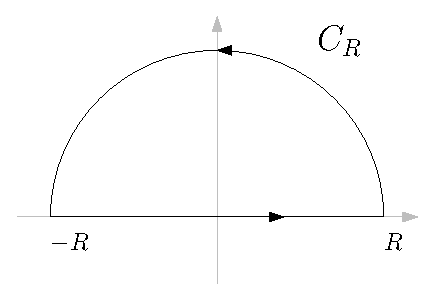
\includegraphics[scale=1]{circ.eps}
    \caption{Полукруг в верхней полуплоскости с обходом против часовой стрелки}
		\label{fig:13.1}
\end{figure}
\\
Пусть 
\begin{align*}
  & I_R = \int_{\gamma_R}f(z)dz = 2 \pi i \left( \us{z_0}{\res} f(z) +  \us{z_1}{\res} f(z)\right) = 2 \pi i \left( \left.\frac{1+z^2}{4z^3}\right|_{z_0} + \left.\frac{1+z^2}{4z^3}\right|_{z_1}\right) = 2 \pi i \cdot \\
  & \cdot \left( \frac{1+\exp\left( \frac{2i \pi}{4} \right)}{4 \exp \left( \frac{3i \pi}{4} \right)} +  \frac{1+\exp\left( \frac{6i \pi}{4} \right)}{4 \exp \left( \frac{9i \pi}{4} \right)}\right) = 2 \pi i \left( \frac{\exp\left( \frac{-i\pi}{4} \right) + \exp\left( \frac{i\pi}{4} \right)}{2 i \cdot 2} +  \frac{\exp\left( \frac{-3i\pi}{4} \right) + \exp\left( \frac{3i\pi}{4} \right)}{-2 i \cdot 2}\right) = \\
  & = \pi \left( \cos \frac{\pi}{4} - \cos \frac{3\pi}{4} \right) = \pi \sqrt{2}
\end{align*}
\begin{align*}
  & \pi \sqrt{2} = \int_{-R}^{+R}f(z) + \int_{C_R}f(z) \us{R\to \infty}{\longrightarrow} \int_{-\infty}^{+\infty} f(z) = \int_{-\infty}^{\infty}f(x)
\end{align*}
Итак, достаточно доказать
\begin{align*}
  & \int_{C_R}f(z)  \us{R\to \infty}{\longrightarrow} 0
\end{align*}
чтобы получить, что $I = \pi \sqrt{2}$.
	\begin{flushright}
    \textit{Лекция 10 (от 06.10)}
\end{flushright}
\Example
Вычисление несобственных интегралов.
\begin{equation}\label{(13.9)}
    I = \int_{-\infty}^{\infty}F_{n,m}(x)dx
\end{equation}
\begin{align*}
  & F_{n,m}(x) = \frac{P_n(x)}{Q_m(x)}, \ Q_m \neq 0 \ \forall x \in \RR, \ m > n+1
\end{align*}
Пусть $R_0 \in (0, R)$,$\gamma_r = [-R;R]\cap C_R$ (см. рис. \ref{fig:13.1}).
Пусть $z_k^+$~--- нули $Q_m(z)$, причем $\Img z_k^+ > 0, \ k \in \{1, \dots,
n\}$, $R_0 = \max \sets{z_k^+}$. Пусть
\begin{align*}
  & I_R = \int_{\gamma_R}F_{n,m}(z)dz = 2 \pi i \sum_{k=1}^n\us{z_k}{\res}F_{n,m}, \ R > R_0
\end{align*}
Но
\begin{align*}
  & I_R = \int_{C_R}F_{n,m}(z)dz + \int_{-R}^RF_{n,m}(z)dz
\end{align*}
Легко заметить, что
\begin{align*}
  & \lim_{R \to \infty} \int_{C_R}F_{n,m}(z)dz = 0
\end{align*}
Значит,
\begin{equation}\label{(13.10)}
    I = \int_{-\infty}^{\infty}F_{n,m}(x)dx = 2 \pi i \sum_{k=1}^n \us{z_k}{\res} F_{n,m}
\end{equation}
\lemma
Пусть $\Phi(z)$ непрерывна на $\sets{z \mid \Img z \geq 0, \abs{z} \geq R_0 >
  0}$.
\\
Пусть $\varepsilon(R) = \max \left\{ \left| \Phi(z) \right| : z \in C_R\right\},
\ R > R_0$. Пусть $\dst \lim_{R \to \infty}R\varepsilon(R) = 0$.
\\
Тогда
\begin{align*}
  & \lim_{R \to \infty }\int_{C_R}\Phi(z)dz = 0
\end{align*}
\pr
\begin{align*}
  & \left| \int_{C_R}\Phi(z)dz \right|\leq \int_{C_R}\left| \Phi(z) \right| dz \leq \varepsilon(R) \int_{C_R}dz = \pi R \varepsilon(R) \us{R \to \infty}{\to} 0
\end{align*}
Применив лемму, докажем равенство \eqref{(13.10)}.
\begin{align*}
  & F_{n,m}(z) = \frac{z^n(1+o(1))}{z^m(1+o(1))}
\end{align*}
\begin{align*}
  & \left| F_{n,m} \right| \leq 2 \left| z \right|^{n-m} \leq 2 R^{n-m}
\end{align*}
\begin{align*}
  & R\varepsilon(R) \leq 2R^{n-m+1} \us{R \to \infty}{\to} 0
\end{align*}
Таким образом доказали формулу \eqref{(13.10)}.
\Example
Вычисление несобственных интегралов.
\begin{equation}\label{(13.11)}
    I = \int_{-\infty}^{\infty}e^{i\alpha x}F_{n,m}(x)dx
\end{equation}
\begin{align*}
  & \alpha > 0, \ F_{n,m}(x) = \frac{P_n(x)}{Q_m(x)}, \ Q_m \neq 0 \ \forall x \in \RR, \ m > n
\end{align*}
Так же, как в предыдущем примере, задаем контур и $R$. По теореме Коши о вычетах
\begin{align*}
  & I_R = \int_{\gamma_R}e^{i\alpha z}F_{n,m}(z) dz = 2 \pi i \sum_{k=1}^n\us{z_k^+}{\res}\left( e^{i\alpha z} F_{n,m}(z)\right)
\end{align*}
Покажем, что
\begin{align*}
  & const = I_R = \int_{C_R}e^{i\alpha z}F_{n,m}(z) dz + \int_{-R}^Re^{i\alpha z}F_{n,m}(z) dz \us{R \to \infty}{\to} \int_{-\infty}^\infty e^{i\alpha z}F_{n,m}(z) dz
\end{align*}
то есть
\begin{equation}\label{(13.12)}
    \lim_{R \to \infty} \int_{C_R}e^{i\alpha z}F_{n,m}(z)dx = 0 \Rightarrow I = 2 \pi i \sum_{k=1}^n \us{z_k^+}{\res}\left( e^{i \alpha z}F_{n,m}(z) \right)
\end{equation}
\lemma (Жордана)
Пусть $\Phi(z)$ непрерывна на $\left\{ z \mid \left| z \right| \geq R_0, \Img z
    \geq 0 \right\}, \ R > R_0$, $C_R$~--- семейство полуокружностей $C_R = \{z
\mid \left| z \right| = R, \Img z \geq 0\}$, $ \varepsilon(R) = \max \left\{
    \left| \Phi(z) \right| : z \in C_R \right\}$, $ \dst \lim_{R \to \infty}
\varepsilon(R) = 0$, $\alpha > 0$. Тогда
\begin{equation}\label{(13.13)}
    \lim_{R \to \infty}\int_{C_R}e^{i \alpha z}\Phi(z)dz = 0
\end{equation}
\pr
$z = x + iy \in C_R$. Значит, положим $x = R \cos \varphi$, $y = R \sin \varphi$,
$ \varphi \in [0,\pi]$. Тогда
\begin{align*}
  & e^{i \alpha z} = e^{i \alpha(x+iy)} = e^{-\alpha y + i \alpha x} = e^{-\alpha R \sin \varphi + i \alpha R \cos \varphi}
\end{align*}
\begin{align*}
  & \left| e^{i \alpha z} \right| = e^{-\alpha R \sin \varphi}
\end{align*}
\begin{align*}
  & z = R e^{i \varphi} \Rightarrow dz = R i e^{i \varphi} d \varphi
\end{align*}
\begin{align*}
  & \left| \int_{C_R}e^{i \alpha z}\Phi(z) dz \right| \leq \int_{0}^{\pi}e^{-\alpha R \sin \varphi}\varepsilon(R) R d \varphi = \varepsilon(R) R \int_{0}^{\pi}e^{-\alpha R \sin \varphi}d \varphi = 2 \varepsilon(R) R \int_{0}^{\frac{\pi}{2}}e^{-\alpha R \sin \varphi}d \varphi \leq \\
  & \leq 2 \varepsilon(R) R \int_{0}^{\frac{\pi}{2}}\exp\left( -\alpha R \frac{2 \varphi}{\pi} \right) d \varphi = \frac{2 \varepsilon(R) R \pi}{2 \alpha R}\left( 1 - e^{-\alpha R} \right) \leq \frac{\pi}{\alpha} \varepsilon(R) \us{R \to \infty}{\to} 0
\end{align*}
Здесь использовали соотношение: $\forall \varphi \in \left[ 0, \dst
    \frac{\pi}{2} \right] \ \sin \varphi \geq \dst \frac{2 \varphi}{\pi}$.
\begin{align*}
  & z = R e^{i \varphi} \Rightarrow dz = R i e^{i \varphi} d \varphi
\end{align*}
Применив лемму, докажем равенство \eqref{(13.12)}. При достаточно больших по
модулю $z$ и $m-n \geq 1$
\begin{align*}
  & \left| F_{n,m}(z) \right| \leq 2 \left| z \right|^{n-m} \leq 2 R^{n-m} \leq \frac{2}{R} \us{R \to \infty}{\to} 0
\end{align*}
\begin{align*}
  & \int_{-\infty}^\infty e^{i \alpha x}F_{n,m}(x) dx = \int_{-\infty}^\infty \cos\alpha xF_{n,m}(x) dx + i \int_{-\infty}^\infty \sin \alpha x F_{n,m}(x) dx
\end{align*}
Таким образом доказали формулу \eqref{(13.12)}.
\section{$\S 14.$ Приращение аргумента $z$ вдоль кривой}
Как известно, $z = x + iy \neq 0 \Rightarrow \Arg z = \left\{\varphi + 2 \pi k
    \mid k \in \ZZ \right\}$. Значит,
\begin{equation}\label{(14.1)}
    \cos \varphi = \frac{x}{\left| z \right|}, \ \sin \varphi = \frac{y}{\left| z \right|}
\end{equation}
\theorem
Пусть $z: [0,1] \mapsto \CC$ непрерывно дифференцируема, $\forall t \in [0,1] \
z(t)\neq 0$. Пусть $\varphi_0 = \varphi(0) \in \Arg z(0)$. Тогда существует и
единственна функция $\varphi: [0,1] \mapsto \RR$, непрерывно дифференцируемая,
$\forall t \in [0,1] \ \varphi(t) \in \Arg z(t)$, т.~е.
\begin{equation}\label{(14.2)}
    \forall t \in [0,1] \ \cos \varphi(t) = \frac{x(t)}{\left| z(t) \right|}, \ \sin \varphi(t) = \frac{y(t)}{\left| z(t) \right|}
\end{equation}
и $\varphi(0) = \varphi_0$, причем $\varphi$ явно вычисляется как
\begin{equation}\label{(14.3)}
    \varphi(t) = \varphi_0 + \int_{0}^t \frac{x(\tau)y'(\tau)-y(\tau)x'(\tau)}{x^2(\tau)+y^2(\tau)}d \tau
\end{equation}
\pr
~
\begin{itemize}
    \item Существование.
    \\
    Рассмотрим \eqref{(14.3)} и покажем, что это решение \eqref{(14.2)}.
    Определим
    \begin{equation}\label{(14.4)}
        \left\{ \begin{matrix}
                u(t) = \cos \varphi(t) \\
                v(t) = \sin \varphi(t)
            \end{matrix} \right. \Rightarrow \left\{ \begin{matrix}
                u'(t) = \varphi'(t)\sin \varphi(t) = -v(t) \varphi'(t) \\
                v'(t) = \varphi'(t)\cos \varphi(t) = u(t) \varphi'(t) 
            \end{matrix} \right.
    \end{equation}
    Определим
    \begin{equation}\label{(14.5)}
        \begin{split}
            & \left\{ \begin{matrix}
                    \tilde{u}(t) = \dst \frac{x(t)}{\left| z(t) \right|} \\
                    \tilde{v}(t) = \dst \frac{y(t)}{\left| z(t) \right|} \\
                \end{matrix} \right. \Rightarrow \\
            & \left\{ \begin{matrix}
                    \dst \frac{d}{dt} \tilde{u}(t) = \dst \frac{d}{dt}\left( \dst \frac{x}{\sqrt{x^2+y^2}} \right) = \dst \frac{x'}{\left| z \right|} - \dst \frac{2x\left( xx'+yy' \right)}{\left| z \right|^3} = -\dst \frac{y}{\left| z \right|} \cdot \dst \frac{xy'-yx'}{x^2+y^2} = - \tilde{v} \dst \frac{xy'-yx'}{x^2+y^2} \\
                    \dst \frac{d}{dt} \tilde{v}(t) = \tilde{u} \dst \frac{xy'-yx'}{x^2+y^2} \\              
                \end{matrix} \right.
        \end{split}
    \end{equation}
    Из \eqref{(14.3)} заметим, что
    \begin{align*}
      \varphi'(t) = \frac{xy'-yx'}{x^2+y^2}
    \end{align*}
    Значит, \eqref{(14.4)} и \eqref{(14.5)} задают одинаковые дифференциальные
    уравнения. Поскольку $\varphi(0) = \varphi_0$ фиксировано. то $u(0) =
    \tilde{u}(0)$, $v(0) = \tilde{v}(0)$ и по теореме единственности $u(t) =
    \tilde{u}(t)$, $v(t) = \tilde{v}(t)$, откуда следует \eqref{(14.2)}.
    \item Единственность.
    \\
    Пусть $\exists \varphi_1(t) \in \Arg z(t)$, непрерывно дифференцируемая,
    $\varphi_1(0) = \varphi_0$ (это равносильно \eqref{(14.2)}); дифференцируя,
    из \eqref{(14.4)} и \eqref{(14.5)} получаем
    \begin{align*}
      \varphi_1'(t) = \frac{xy'-yx'}{x^2+y^2}
    \end{align*}
    а значит, эта функция находится по формуле \eqref{(14.3)} и совпадает с
    $\varphi$.
\end{itemize}
\note
Формулу \eqref{(14.3)} можем записать как
\begin{equation}\label{(14.6)}
    \varphi(t) = \varphi_0 + \Img \int_{0}^t \frac{z'(\tau)}{z(\tau)}d \tau
\end{equation}
\pr
\begin{align*}
  & \frac{z'}{z} = \frac{\left( x'+iy' \right)\left( x-iy \right)}{\left( x+iy \right)\left( x-iy \right)} = \frac{x'x+y'y+i\left( xy'-x'y \right)}{x^2+y^2}
\end{align*}
\begin{align*}
  & \Img \frac{z'}{z} = \Img \frac{x'x+y'y+i\left( xy'-x'y \right)}{x^2+y^2} = \frac{xy'-x'y}{x^2+y^2}
\end{align*}
\Def
\textbf{Приращением аргумента $z$ вдоль кривой $z(t)$} на отрезке $[0,1]$
называется
\begin{equation}\label{(14.7)}
    \Delta_{[0,1]}\argt z = \varphi(1) - \varphi(0) = \Img \int_{0}^1 \frac{z'(\tau)}{z(\tau)}d \tau
\end{equation}
\begin{figure}[h!]
		\centering
		\includegraphics[scale=0.8]{deltaarg.eps}
    \caption{Приращение аргумента вдоль кривой}
		\label{fig:14.1}
\end{figure}\\
\theorem (логарифмическое свойство)
Пусть $z(t) \in C^1[0;1]$, $\forall t \in [0,1] \ z(t) \neq 0$. Пусть $z(t) =
z_1(t)z_2(t)$, $z_k(t) \in C^1[0,1]$. Тогда
\begin{equation}\label{(14.8)}
    \Delta_{[0,1]}\argt z = \Delta_{[0,1]}\argt z_1 + \Delta_{[0,1]}\argt z_2
\end{equation}
\pr
Из \eqref{(14.7)} имеем:
\begin{align*}
  & \Delta_{[0,1]} \argt z(t) = \Img \int_{0}^{1}\frac{\left( z_1(\tau)z_2(\tau) \right)'}{z_1(\tau)z_2(\tau)}d \tau =\Img \int_{0}^{1}\frac{z_1'z_2+z_1z_2'}{z_1z_2}d \tau = \Img \int_{0}^{1}\frac{z_1'}{z_1}d \tau + \Img \int_{0}^{1}\frac{z_2'}{z_2}d \tau = \\
  & = \Delta_{[0,1]} \argt z_1(t) + \Delta_{[0,1]} \argt z_2(t) 
\end{align*}
\Def
Пусть $\gamma$~--- кривая в $\CC$, заданная параметризацией $z=z(t)$, $t \in
[0;1]$, $z \in C^1[0;1]$, $0 \not \in \gamma$. Тогда \textbf{приращением
  аргумента $z$ вдоль кривой $\gamma$} называется
\begin{equation}\label{(14.9)}
    \Delta_{\gamma}\argt z = \Delta_{[0;1]}\argt z = \Img \int_{0}^1 \frac{z'(\tau)}{z(\tau)}d \tau
\end{equation}
Определение корректно, т.~к. \eqref{(14.9)} равносильно
\begin{equation}\label{(14.10)}
    \Delta_{\gamma}\argt z = \Img \int_{\gamma} \frac{dz}{z}
\end{equation}
	\begin{Def}
	Векторным полем на $D$ называется функция $\vec{a}: D\to\R^n$.\\ $\vec{a}=a^1\vec{e_1}+\ldots+a^n\vec{e_n}$.
	Если $(\vec{e_1}, \ldots, \vec{e_n})$ --- ортонормированный базис евклидова пространства $\R^n$, то операции соответствия векторных полей и дифференциальных форм валентности $n$ определяются так: $(\vec{a})^\sharp=a_1(x)dx^1+\ldots+a_n(x)dx^n$ и для $\Omega(x)=w_1(x)dx^1+\ldots+w_n(x)dx^n$, $(\Omega)^\flat=w^1(x)\vec{e_1}+\ldots+w^n(x)\vec{e_n}$, где $a_i(x)=a^i(x), w_i(x)=w^i(x), i=1,\ldots, n, (dx^1, \ldots, dx^n)$ --- сопряженный базис к $(\vec{e_1}, \ldots, \vec{e_n})$.
	
	Аналогично определяются операции соответствия для поливекторных полей и дифференциальных форм произвольной валентности.
\end{Def}

\subsubsection{Основные операции теории поля.}
По сути все основные операции теории поля --- это дифференцирование дифференциальных форм.

Начнем с $0$-формы $f(x)$ в $\R^n:$
\begin{align*}
	df&=\dfrac{\partial f}{\partial x^1}dx^1+\ldots+\dfrac{\partial f}{\partial x^n}dx^n \\
	(df)^\flat&= \dfrac{\partial f}{\partial x^1}e_1+\ldots+\dfrac{\partial f}{\partial x^n}e_n=\grad f
\end{align*}

$1$-форма в $\R^3$:
$$
	(\vec{a})^\sharp= a_1(x)dx^1+a_2(x)dx^2+a_3dx^3=Pdx+Qdy+Rdz
$$
\begin{multline*}
	d(\vec{a})^\sharp=dP\wedge dx+dQ\wedge dy+dR\wedge dz=
	\\
	=\left(\dfrac{\partial P}{\partial x}dx+\dfrac{\partial P}{\partial y}dy+\dfrac{\partial P}{\partial z}dz \right)\wedge dx+\\+\left(\dfrac{\partial Q}{\partial x}dx+\dfrac{\partial Q}{\partial y}dy+\dfrac{\partial Q}{\partial z}dz \right)\wedge dy+\\+\left(\dfrac{\partial R}{\partial x}dx+\dfrac{\partial R}{\partial y}dy+\dfrac{\partial R}{\partial z}dz \right)\wedge dz=
	\\
	=\left(\dfrac{\partial R}{\partial y}-\dfrac{\partial Q}{\partial z}\right)dy\wedge dz+\left(\dfrac{\partial P}{\partial z}-\dfrac{\partial R}{\partial x}\right)dz\wedge dx+\left(\dfrac{\partial Q}{\partial x}-\dfrac{\partial P}{\partial y}\right)dx\wedge dy
\end{multline*}
$$*d(\vec{a})^\sharp = \left(\dfrac{\partial R}{\partial y}-\dfrac{\partial Q}{\partial z}\right)dx+\left(\dfrac{\partial P}{\partial z}-\dfrac{\partial R}{\partial x}\right)dy+\left(\dfrac{\partial Q}{\partial x}-\dfrac{\partial P}{\partial y}\right)dz$$
$$(*d(\vec{a})^\sharp)^\flat = \left(\dfrac{\partial R}{\partial y}-\dfrac{\partial Q}{\partial z}\right)\vec{i}+\left(\dfrac{\partial P}{\partial z}-\dfrac{\partial R}{\partial x}\right)\vec{j}+\left(\dfrac{\partial Q}{\partial x}-\dfrac{\partial P}{\partial y}\right)\vec{k}:=\rot\vec{a}$$

$(n-1)$-форма в $\R^n$:

$*(\vec{a})^\sharp=*(a_1(x)dx^1+\ldots+a_n(x)dx^n)=a_1(x)dx^2\wedge\ldots\wedge dx^n+\ldots+(-1)^{n-1}a_n(x)dx^1\wedge\ldots\wedge dx^{n-1}$.
\begin{multline*}
	d(*(\vec{a})^\sharp)=da_1(x)\wedge dx^2\wedge\ldots\wedge dx^n+\ldots+(-1)^{n-1}da_n(x)\wedge dx^1\wedge\ldots\wedge dx^{n-1}=\\=\dfrac{\partial a_1(x)}{\partial x^1}dx^1\wedge\ldots\wedge dx^n+\ldots+\dfrac{\partial a_n(x)}{\partial x^n}dx^1\wedge\ldots\wedge dx^n=\left(\dfrac{\partial a_1(x)}{\partial x^1}+\ldots + \dfrac{\partial a_n(x)}{\partial x^n}\right)dx^1\wedge\ldots\wedge dx^n.
\end{multline*}
$*d(*(\vec{a})^\sharp)=\dfrac{\partial a_1(x)}{\partial x^1}+\ldots+\dfrac{\partial a_n(x)}{\partial x^n}=\di\vec{a}$ --- дивергенция.

\begin{example}
	\begin{align*}
		\rot(\grad f)&=(*(d(\grad f)^\sharp))^\flat=(*(d(df)))^\flat=0\\
		\di(\rot\vec{a})&=*(d(*(\rot\vec{a})^\sharp))=*(d(**d(\vec{a}^\sharp)))=0
	\end{align*}
\end{example}

Векторный дифференциальный оператор набла: \fbox{$\nabla:=\left(\dfrac{\partial}{\partial x},\dfrac{\partial}{\partial y}, \dfrac{\partial}{\partial z}\right)$}.

\begin{align*}
	\grad f&= \left(\dfrac{\partial f}{\partial x}, \dfrac{\partial f}{\partial y}, \dfrac{\partial f}{\partial z}\right)=\nabla f\\
	\di\vec{a}&=\dfrac{\partial P}{\partial x}+\dfrac{\partial Q}{\partial y}+\dfrac{\partial R}{\partial z}=(\nabla, \vec{a})\\
	\rot\vec{a}&=[\nabla, \vec{a}]=
	\begin{vmatrix}
		\vec{i} & \vec{j} & \vec{k}\\
		\frac{\partial}{\partial x} & \frac{\partial}{\partial y} & \frac{\partial}{\partial z}\\
		P & Q & R
	\end{vmatrix}
\end{align*}


\begin{Def}
	$p$-форма $\Omega$ называется замкнутой, если $d\Omega=0$. $p$-форма $\Omega$ называется точной, если существует $(p-1)$-форма $\Pi$, такая что $\Omega=d\Pi$.
\end{Def}

\begin{corollary}
	Каждая точная форма замкнута. 
\end{corollary}

\begin{proof}
	Пусть $\Omega$ --- точная форма. Следовательно $\Omega=d\Pi\Rightarrow d\Omega=d(d\Pi)=0\Rightarrow\Omega$ --- замкнутая.
\end{proof}

\begin{Def}
	Область $D\subset\R^n$ называется звездной, если $\exists x_0\in D$, такое, что \\$ \varphi(x, t)=x_0+(1-t)(x-x_0)$, непрерывное отображение из $D\times[0,1]$ в $D$ и такое, что $\varphi(x,0)=x\ \ \forall x\in D, \varphi(x,1)=x_0\ \ \forall x\in D.$
	
	$\varphi$ --- называется прямым стягиванием $D$ в точку $x_0$.
\end{Def}

\subsubsection{Операция замены переменных в дифференциальной форме.}
\begin{Def}
	Пусть $\Omega(x)$ --- дифференциальная $p$-форма в области $U\subset\R^n, \varphi:V\to U$ --- диффеоморфизм области $V\subset\R^n$ на $U, x=\varphi(x).
	\\ \varphi^*\Omega(y)$ --- дифференциальная $p$-форма в области $V$, определяемая на любом наборе $p$ векторов из $\R^n, b_1,\ldots, b_p$, как  $\varphi^*\Omega(y)(b_1, \ldots, b_p)=\Omega(\varphi(y))(\varphi'(y)b_1, \ldots, \varphi'(y)b_p)$, где $\varphi'(y)$ --- это матрица Якоби отображения $\varphi$.
\end{Def} 

Пусть $\Omega(x)=w(x)dx^{i_1}\wedge\ldots\wedge dx^{i_p}$.

$(\varphi^*\Omega)(y)(b_1,\ldots, b_p)=w(\varphi(y))dx^{i_1}\wedge\ldots\wedge dx^{i_p}(\varphi'(y)b_1,\ldots, \varphi'(y)b_p)=w(\varphi(y))\det((\varphi'(y)b_j)^{i_k})_{j=1,k=1}^{p,p}$

Проверим, что $(\varphi^*\Omega)(y)=w(\varphi(y))d\varphi^{i_1}(y)\wedge\ldots\wedge d\varphi^{i_p}(y)$.

Подсчитаем 
\begin{multline*}
	w(\varphi(y))d\varphi^{i_1}(y)(b_1, \ldots, b_p)=w(\varphi(y))det(d\varphi^{i_k}(y)(b_j))_{j=1,k=1}^{p,p}=\\=w(\varphi(y))\det((\varphi'(y)d_j)^{i_k})_{j=1,k=1}^{p,p}\text{, так как }\\d\varphi^{i_k}(y)(b_j) = \sum\limits_{l=1}^n\dfrac{\partial \varphi^{i_k}}{\partial y^l}(y)(b_j^l)=(\varphi'(y)b_j)^{i_k}.
\end{multline*}

Правило подсчета $\varphi^*:$ если $\Omega(x)=\sum\limits_{1\leqslant i_1<\ldots<i_p\leqslant n}w_{i_1\ldots i_p}(x)dx^{i_1}\wedge\ldots\wedge dx^{i_p}$, то\\ 
$\varphi^*\Omega(y)=\sum\limits_{1\leqslant i_1<\ldots<i_p\leqslant n}w_{i_1\ldots i_p}(\varphi(y))d\varphi^{i_1}(y)\wedge\ldots\wedge d\varphi^{i_p}(y)$.
\subsubsection{Свойства операции замены переменных.}

\begin{enumerate}
	\item $\varphi^*(\alpha\Omega+\beta\Pi)=\alpha\varphi^*\Omega+\beta\varphi^*\Pi$
	\item
	$\varphi^*(\Omega\wedge\Pi)=\varphi^*(\Omega)\wedge\varphi^*(\Pi)$
	\item
	$\varphi^*(d\Omega)=d(\varphi^*\Omega)$
	\item 
	$\varphi^*\psi^*\Omega=(\varphi\psi)^*\Omega$
\end{enumerate}

\begin{proof}\ 
	\begin{enumerate}
		\item очевидно.
		\item\begin{multline*}
			\varphi(\Omega\wedge\Pi)=\\=\varphi^*\left(\sum\limits_{1\leqslant i_1<\ldots<i_p\leqslant n}\sum\limits_{1\leqslant j_1<\ldots<j_q\leqslant n}w_{i_1\ldots i_p}(x)\varpi_{j_1\ldots j_q}(x)dx^{i_1}\wedge\ldots\wedge dx^{i_p}\wedge dx^{j_1}\wedge\ldots\wedge dx^{j_q}\right)=\\=\sum\limits_{1\leqslant i_1<\ldots<i_p\leqslant n}\sum\limits_{1\leqslant j_1<\ldots<j_q\leqslant n}w_{i_1\ldots i_p}(\varphi(y))\varpi_{j_1\ldots j_q}(\varphi(y))d\varphi^{i_1}(y)\wedge\ldots\wedge d\varphi^{i_p}(y)\wedge \\ \wedge d\varphi^{j_1}(y)\wedge\ldots\wedge d\varphi^{j_q}(y)=\varphi^*(\Omega)\wedge \varphi^*(\Pi).
		\end{multline*} 
		\item 
		\begin{multline*}
			d\Omega(x)=\sum\limits_{1\leqslant i_1<\ldots<i_p\leqslant n}dw_{i_1\ldots i_p}(x)\wedge dx^{i_1}\wedge\ldots\wedge dx^{i^p}=
			\\
			=\sum\limits_{1\leqslant i_1<\ldots<i_p\leqslant n}\sum\limits_{k=1}^n\dfrac{\partial w_{i_1\ldots i_p}}{\partial x^k}(x)dx^{k}\wedge dx^{i_1}\wedge\ldots\wedge dx^{i_p}
		\end{multline*}
		$\varphi^*d\Omega(x)=\sum\limits_{1\leqslant i_1<\ldots<i_p\leqslant n}\sum\limits_{k=1}^n\dfrac{\partial w_{i_1\ldots i_p}}{\partial x^k}(\varphi(y))d\varphi^k(y)\wedge d\varphi^{i_1}(y)\wedge\ldots\wedge d\varphi^{i_p}(y)$
		
		$\varphi^*\Omega(y) = \sum\limits_{1\leqslant i_1<\ldots<i_p\leqslant n} w_{i_1\ldots i_p}(\varphi(y))d\varphi^{i_1}(y)\wedge\ldots\wedge d\varphi^{i_p}(y)$
		\begin{multline*}
			d\varphi^*\Omega(y)=\sum\limits_{1\leqslant i_1<\ldots<i_p\leqslant n}(dw_{i_1\ldots i_p}(\varphi(y))d\varphi^{i_1}(y)\wedge\ldots\wedge d\varphi^{i_p}(y)+\\+w_{i_1\ldots i_p}(\varphi(y))\underbrace{d(d\varphi^{i_1}(y)\wedge\ldots\wedge d\varphi^{i_p})}_{=0})
		\end{multline*}
	\item $\Omega=w(x)dx^{i_1}\wedge\ldots\wedge dx^{i_p}$ \\
	$\psi^*\Omega=w(\psi(y))d\psi^{i_1}(y)\wedge\ldots\wedge d\psi^{i_p}(y)$ \\
	$\varphi^*\psi^*\Omega=w(\psi(\varphi(z)))d\psi^{i_1}(\varphi(z))\wedge\ldots\wedge d\psi^{i_p}(\varphi(z))=(\varphi\psi)^*\Omega$
	\end{enumerate}
\end{proof}

\begin{Def}
	Область $G\subset\R^n$ называется звездообразной, если она является диффеоморфным образом звездной области.
\end{Def}

Если $\Omega$ --- дифференциальная форма в $D\times[0,1]$, то $\varphi^*\Omega$--- дифференциальная форма в $D$, где $\varphi$ --- прямое стягивание звездной области $D$, то $p$-форма $\Omega$ состоит из слагаемых вида $a(x,t)dx^{i_1}\wedge\ldots\wedge dx^{i_p}$ и $b(x,t)dt\wedge dx^{i_1}\wedge\ldots\wedge dx^{i_{p-1}}$.

$\Omega(x,t_0)$ при фиксированном $t_0$ будем считать дифференциальной формой на $D, dt\equiv 0$.

\begin{lemma}
	Если $\Omega$ --- гладкая $p$-форма в $D\times[0,1]$, то $(dK\Omega+Kd\Omega)(x)=\Omega(x,1)-\Omega(x,0)$, где $K$ --- линейная операция, заданная на базисных слагаемых как $K(a(x,t)dx^{i_1}\wedge\ldots\wedge dx^{i_p})=0,K(b(x,t)dt\wedge dx^{i_1}\wedge\ldots\wedge dx^{i_{p-1}})=\left(\int\limits_{0}^1b(x,t)d\mu(t)\right)\wedge dx^{i_1}\wedge\ldots\wedge dx^{i_{p-1}}$.
\end{lemma}

\begin{proof}\ 
	\begin{enumerate}
		\item На $a(x,t)dx^{i_1}\wedge\ldots\wedge dx^{i_{p}}: K\Omega=0, \\d\Omega=\dfrac{\partial a(x,t)}{\partial t}dt\wedge dx^{i_1}\wedge\ldots\wedge dx^{i_{p}}+\sum\limits_{k=1}^n\dfrac{\partial a(x,t)}{\partial x^k}dx^k\wedge dx^{i_1}\wedge\ldots\wedge dx^{i_{p}}$;\\ $Kd\Omega=\left(\int\limits_{0}^1\dfrac{\partial a(x,t)}{\partial t}d\mu(t)\right)dx^{i_1}\wedge\ldots\wedge dx^{i_p}=(a(x, 1)-a(x,0))dx^{i_1}\wedge\ldots\wedge dx^{i_p}\Rightarrow\\ (dK\Omega+kd\Omega)(x)=\Omega(x,1)-\Omega(x,0)$.
		\item При $b(x,t)dt\wedge dx^{i_1}\wedge\ldots\wedge dx^{i_{p-1}}=\Omega:\\ K\Omega=\left(\int\limits_{0}^1b(x,t)d\mu(x)\right)\wedge dx^{i_1}\wedge\ldots\wedge dx^{i_{p-1}}=\sum\limits_{k=1}^n \int\limits_{0}^1 \dfrac{\partial b(x,t)}{\partial x^k}d\mu(t)dx^k\wedge dx^{i_1}\wedge\ldots\wedge dx^{i_{p-1}}$
		$d\Omega=db(x,t)\wedge dt\wedge dx^{i_1}\wedge\ldots\wedge dx^{i_{p-1}}=\sum\limits_{k=1}^n\dfrac{\partial b(x,t)}{\partial x^k}dx^k\wedge dx^{i_1}\wedge\ldots\wedge dx^{i_{p-1}}=\\=-\sum\limits_{k=1}^n\dfrac{\partial b(x,t)}{\partial x^k}dt\wedge dx^k\wedge dx^{i_1}\wedge\ldots\wedge dx^{i_{p-1}}$\\
		$Kd\Omega=-\sum\limits_{k=1}^n\left(\int\limits_{0}^1 \dfrac{\partial b(x,t)}{\partial x^k}d\mu(t)\right)dx^k\wedge dx^{i_1}\wedge\ldots\wedge dx^{i_{p-1}}$\\
		$dK\Omega+Kd\Omega=0=\Omega(x,1)-\Omega(x,0)$
	\end{enumerate}
\end{proof}

\begin{theorem}(Лемма Пуанкаре)
	Каждая замкнутая в звездообразной области $D$ гладкая форма точна в ней.
\end{theorem}

\begin{proof}
	Пусть $D$ --- звездная область, $\varphi$ --- прямое стягивание. Рассмотрим $\varphi^*\Omega$ в $D\times[0,1]$. $\Omega$ --- замкнута $\Rightarrow d\Omega=0\Rightarrow d\varphi^*\Omega=\varphi^*d\Omega=0\Rightarrow \varphi^*\Omega$ --- замкнута в $D\times[0,1]$. Тогда по лемме $dK\varphi^*\Omega=-Kd\varphi^*\Omega+\varphi^*\Omega(x,1)-\varphi^*\Omega(x,0)$.
	
	$\Omega=\sum\limits_{1\leqslant i_1 < \ldots < i_p \leqslant n}w_{i_1\ldots i_p}(y)dy^{i_1}\wedge\ldots\wedge dy^{i_p}$, заменим переменную $y=\varphi(x,t)$,
	
	$\varphi^*\Omega=\sum\limits_{1\leqslant i_1 < \ldots < i_p \leqslant n} w_{i_1\ldots i_p}(\varphi(x,t))d\varphi^{i_1}(x,t)\wedge\ldots\wedge d\varphi^{i_p}(x,t)$,
	
	$d\varphi^{j}(x,t)=-(x^j-x_0^j)dt+(1-t)dx^j$. Считаем $dt\equiv0$, значит все слагаемые в которых появятся $dt$ обнулятся.
	
	$\varphi^*\Omega(x,1) =0$
	
	$\varphi^*\Omega(x,0)=\sum\limits_{1\leqslant i_1 < \ldots < i_p \leqslant n}w_{i_1\ldots i_p}(x)dx^{i_1}\wedge\ldots\wedge dx^{i_p}=\Omega(x)$. 
	
	Итого $dK\varphi^*\Omega=-\Omega(x)\Rightarrow \Omega(x)=d\Pi(x)$, где $\Pi(x)=-K\varphi^*\Omega$
	
	Пусть $D=\psi(G)$, где $G$ --- звездная область, $\psi$ --- диффеоморфизм. В $D$ есть замкнута форма $\Omega$. Рассмотрим $\psi^*\Omega$ --- форма в $G$, она замкнута, так как $d\psi^*\Omega=\psi^*d\Omega=0$. $G$ --- звездная область и по уже доказанному $\Pi=-K\varphi^*\psi^*\Omega$ является первообразной, то есть $d\Pi=\psi^*\Omega$. Тогда для $(\psi^{-1})^*\Pi$ справедливо $d(\psi^{-1})^*\Pi=(\psi^{-1})^*d\Pi=(\psi^{-1})^*\psi^*\Omega=\Omega$, в предположении, что $\varphi^*\psi^*\Omega=(\varphi\psi)^*\Omega$.
\end{proof}

\begin{Def}
	Векторное поле называется потенциальным, если оно является градиетном некоторой функции(скалярного поля), которое называется его потенциалом.
	
	$\vec{a}=\grad f, \vec{a}$ --- потенциальное поле, $f$ --- потенциал ($f+C$ --- тоже потенциал).
\end{Def}

\begin{Def}
	Векторное поле называется солениодальным, если оно является ротором некоторого векторного поля, которое называется векторным потенциалом исходного поля.
	
	$\vec{a}=\rot\vec{b}, \vec{a}$ --- соленоидальное поле, $\vec{b}$ --- векторный потенциал ($\vec{b}+\grad f$ --- тоже  векторный потенциал, так как $\rot\grad f=0$).
\end{Def}

\begin{corollary}[из определения]
	Если $\vec{a}$ --- потенциальное поле, то $\rot\vec{a}=\vec{0}$. Если $\vec{a}$ --- соленоидальное поле, то $\di\vec{a}=0$.
\end{corollary}

\begin{corollary}[из леммы Пуакаре]
	Если $\rot\vec{a}=0$ в звездообразной области $D$, то гладкое векторное поле $\vec{a}$ является потенциальным. Если $\di\vec{a}=0$ в звездообразной области $D$, то гладкое векторное поле $\vec{a}$ является соленоидальным.
\end{corollary}

\subsection{Интегрирование дифференциальных форм.}

Пространство $\Lambda_n(\R^n)$ одномерно. Если $(f^1,\ldots, f^n)$ --- базис $E^*$, то\\ $\{cf^1\wedge\ldots\wedge f^n:c\in\R^n\}=\Lambda_n(\R^n)$.

Пусть $(e_1^0,\ldots,e_n^0)$ --- ортонормированный базис $E$. $(e_1,\ldots, e_n)$ --- другой базис, $e_j=t^i_je_i^0$, $T$ --- матрица перехода.

$V_{e^0}:=dx^1_0\wedge\ldots\wedge dx^n_0$ --- базисный элемент пространства $n$-форм в любой точке области $D$.

$V_e:=dx^1\wedge\ldots\wedge dx^n$.

$V_{e^0}(e_1,\ldots, e_n)=dx^1_0\wedge\ldots\wedge dx^n_0(e_1,\ldots, e_n)=\det(dx_0^i(e_j))_{i=1,j=1}^{p,p}=\det T$.

$V_e(e_1,\ldots, e_n)=dx^1\wedge\ldots\wedge dx^n(e_1,\ldots, e_n)=1$.

\begin{prop}
	$V_{e^0}=\det TV_e$.
\end{prop}

\begin{Def}
	Два базиса называются эквивалентными, если $\det T>0$, где $T$ --- матрица перехода от одного базиса к другому.
\end{Def}

\begin{prop}
	Отношение эквивалентности базисов --- отношение эквивалентности на множестве базисов. Значит все базисы разбиваются на 2 класса эквивалентности. Задается ориентация базисов.
\end{prop}

Форма $V_e$ позволяет определить ориентацию базиса. Она назывется формой ориентированного объема.

Введем обозначение: $\Pi=\{0<x^i<1:i=1,\ldots,n\}$ --- призма, натянутая на векторы $e_1, \ldots, e_n$.

\begin{prop}
	$V_{e^0}=\pm \mu(\Pi)$, где $+$ соответствует положительно определенному относительно $(e_1^0,\ldots,e^0_n)$ базису $(e_1,\ldots, e_n)$.
\end{prop}




























	Дифференциальную форму валентности $n$ в $D\subset\R^n$ можно записать в виде $\Omega(x)=\alpha(x)V_{e^0}$, так как пространство полилинейных форм валентности $n$ в $n$-мерном пространстве одномерное.

\begin{Def}
	Интегралом от формы $\Omega(x)=\alpha(x)V_{e^0}$ по области $D\subset\R^n$ называется $\int\limits_{D}\Omega=\int\limits_{D}\alpha(x)d\mu(x)$, где $\alpha$ --- суммируемая на $D$.
\end{Def}

\begin{prop}
	Если $\varphi:G\to D$ --- гладкое отображение области $G\subset \R^n$ на $D$, такое, что $\det \varphi'(u)\ne 0\ \ \forall u\in G$ (то есть $\varphi$ --- неособое), то $\int\limits_{G}\varphi^*\Omega=\pm\int\limits_{D}\Omega$
\end{prop}

\begin{proof}
	\begin{multline*}
		\varphi^*\Omega(u)(H_1,\ldots, H_n)=\Omega(\varphi(u))(\varphi'(u)H_1, \ldots, \varphi'(u)H_n)=\\=\alpha(\varphi(u))V_{e^0}(\varphi'(u)H_1, \ldots, \varphi'(u)H_n)=\alpha(\varphi(u))dx_0^1\wedge\ldots\wedge dx^n_0(\varphi'(u)H_1, \ldots, \varphi'(u)H_n)=\\=\alpha(\varphi(u))\det((\varphi'(u)H_i)^j)=\alpha(\varphi(u))\det\varphi'(u)det(H^j_i)=\alpha(\varphi(u))\det\varphi'(u)\widetilde{V_{e^0}}(H_1,\ldots,H_n).
	\end{multline*}
	
	$\int\limits_{G}\varphi^*\Omega=\int\limits_{G}\alpha(\varphi(u))\det\varphi'(u)d\mu(u)$.
	
	$\int\limits_{D}\Omega=\int\limits_{D}\alpha(x)d\mu(x)=[x=\varphi(x)]=\int\limits_{G}\alpha(\varphi(u))|\det\varphi'(u)|d\mu(u)=\pm\int\limits_{G}\alpha(\varphi(u))\det\varphi'(u)d\mu(u)$
\end{proof}

\begin{Def}
	Стандартным кубом $K$ называется множество $\{0<x^i_0<1\},i=1,\ldots,n$ в ортонормированном базисе $e^0_1,\ldots,e_n^0$.
	
	Цепь стандартных кубов --- это линейная комбинация $\Pi=\sum\limits_{j=1}^mn_jK_j$, где $n_j\in \Z, K_j$ --- стандартные кубы.
\end{Def}

\begin{Def}
	Интеграл от $n$-формы $\Omega$ по цепи кубов определяется как $\int\limits_{\Pi}\Omega=\sum\limits_{j=1}^m n_j\int\limits_{K_j}\Omega$
\end{Def}

Граница стандартного куба --- цепь стандартных $(n-1)$-мерных кубов.

$\partial K=\sum\limits_{j=1, \alpha=0,1}^m\varepsilon_j^\alpha K_{j,\alpha},\ \ K_{j,\alpha}=\{0<x_0^i<1;i\ne j, x_0^j=\alpha\}$.

Правило ориентации граней куба: грань $K_{j,\alpha}$ ориентирована положительным базисом пространства $E_j=\{(x_0^1,\ldots,x_0^{j-1},x_0^{j+1},\ldots,x_0^n)\}$ таким, что дополнив его первым вектором, являющимся нормалью к грани $K_{j,\alpha}$, выходящей из куба $K$, получим положительный базис $\R^n$.













\end{document}